\begin{savequote}
%``Fluid mechanics is especially rich in non-linearities''
%\qauthor{W.F. Ames}

``As a result of these discussions, I developed an intense fear of flows in which contact discontinuities were a possibility''
\qauthor{S.K. Godunov, Reminiscences about difference schemes. J Comp Phys, 153:1-5, 1999}

``The first obstacle may be one of sentiment. It is said that in a certain
grassy part of the world a man will walk a mile to catch a horse, whereon to
ride a quarter of a mile to pay an afternoon call. Similarly, it is not quite
respectable to arrive at a mathematical destination, under the gaze of a
learned society, at the mere foot pace of arithmetic. Even at the expense of
considerable time and effort, one should be mounted on the swift steed of
symbolic analysis.

The following notes are written for those who desire to arrive by the easiest
route, and who are not self-conscious about the respectability of their means
of locomotion.''

\qauthor{Lewis F. Richardson, How to solve differential equations approximately
by arithmetic, Mathl. Gaz., 12:415-21, 1925.}

\end{savequote}

\chapter{Numerical Method}
\label{NumericalMethod}

%\minitoc

In this Chapter we present the numerical method used to solve the equations of
ideal magnetohydrodynamics. The various numerical methods contained in the code,
ATLAS are described, including
the method for constraining the divergence of the magnetic field equal to zero, 
the Godunov method for capturing shocks,
the corner transport upwind method for describing multidimensional flows,
the atomic radiative cooling losses,
the parallel structure and finally the method for adaptively refining the mesh in
order to give highest resolutions in regions where shocks occur.
A description of the computer cluster, Leda, built to perform some of the calculations
in this thesis is given.

\section{The Equations of Ideal Magnetohydrodynamics (MHD)}
\label{EquationsofIdealMagnetohydrodynamicsMHD}
%The simulation code solves the ideal magnetohydrodynamics (MHD) equations. 
%These equations can be derived by taking zeroth, first and second velocity moments of the Boltzmann equation.

The ideal MHD equations are in terms of the eight variables in addition to time t which are conserved in a volume: 
density $\rho$, momentum, $\rho \mathbf u$, magnetic flux density $\mathbf B$ and energy density, $E$.
These equations expressed in conservation form are as follows:

\noindent
Conservation of Mass:
\begin{equation}
\frac{\partial \rho}{\partial t}+\boldsymbol{\nabla}\cdot(\rho \mathbf u)=0
\end{equation}
Conservation of Momentum:
\begin{equation}
\frac{\partial}{\partial t}\left(
\rho \mathbf u
\right)
+\boldsymbol{\nabla}
\cdot
\left[
\rho \mathbf u \otimes \mathbf u
+\left(
p^*
\right)
\mathbf{{\overline {\overline I}}}
+\mathbf{B} \otimes \mathbf{B}
\right]
=0
\end{equation}
Conservation of Flux:
\begin{equation}
\frac{\partial \mathbf{B} }{\partial t}+
\boldsymbol{\nabla}
\cdot
(
\mathbf{u} \otimes \mathbf{B}-
\mathbf{B} \otimes \mathbf{u})
= 0
\end{equation}
Conservation of Energy:
\begin{eqnarray}
\frac{\partial E}{\partial t}
+\boldsymbol{\nabla}
\cdot
\left[
\left( E + p^*\right) \mathbf{u}
- (\mathbf{u}\cdot\mathbf{B})\mathbf{B}
\right] + L_{cooling} = 0
\end{eqnarray}
where $E$ is the total energy, kinetic, internal and magnetic 
\begin{equation}
E =
\frac{1}{2}\rho |\mathbf{u}|^2 + 
\frac{p}{\gamma-1}+
\frac{1}{2} |\mathbf{B}|^2
\end{equation}
and $p^*$ is the sum of thermal and magnetic pressure:
\begin{equation}
p^* = p + \frac{1}{2}|\mathbf{B}|^2
\end{equation}
$L_{cooling}$ is the loss of energy due to cooling.
The units are chosen so that $\mathbf B$ absorbs a factor of $1/\sqrt {4 \pi}$.
The adiabatic index is $\gamma = 5/3$ for a monatomic gas throughout the simulations.
$\mathbf{I}$ is the identity tensor.
There are eight equations and nine variables. In order to close the system one more equation is required, the equation of state.
The equation of state is chosen to be the ideal gas equation.



%\begin{figure}[t]
%\centering
%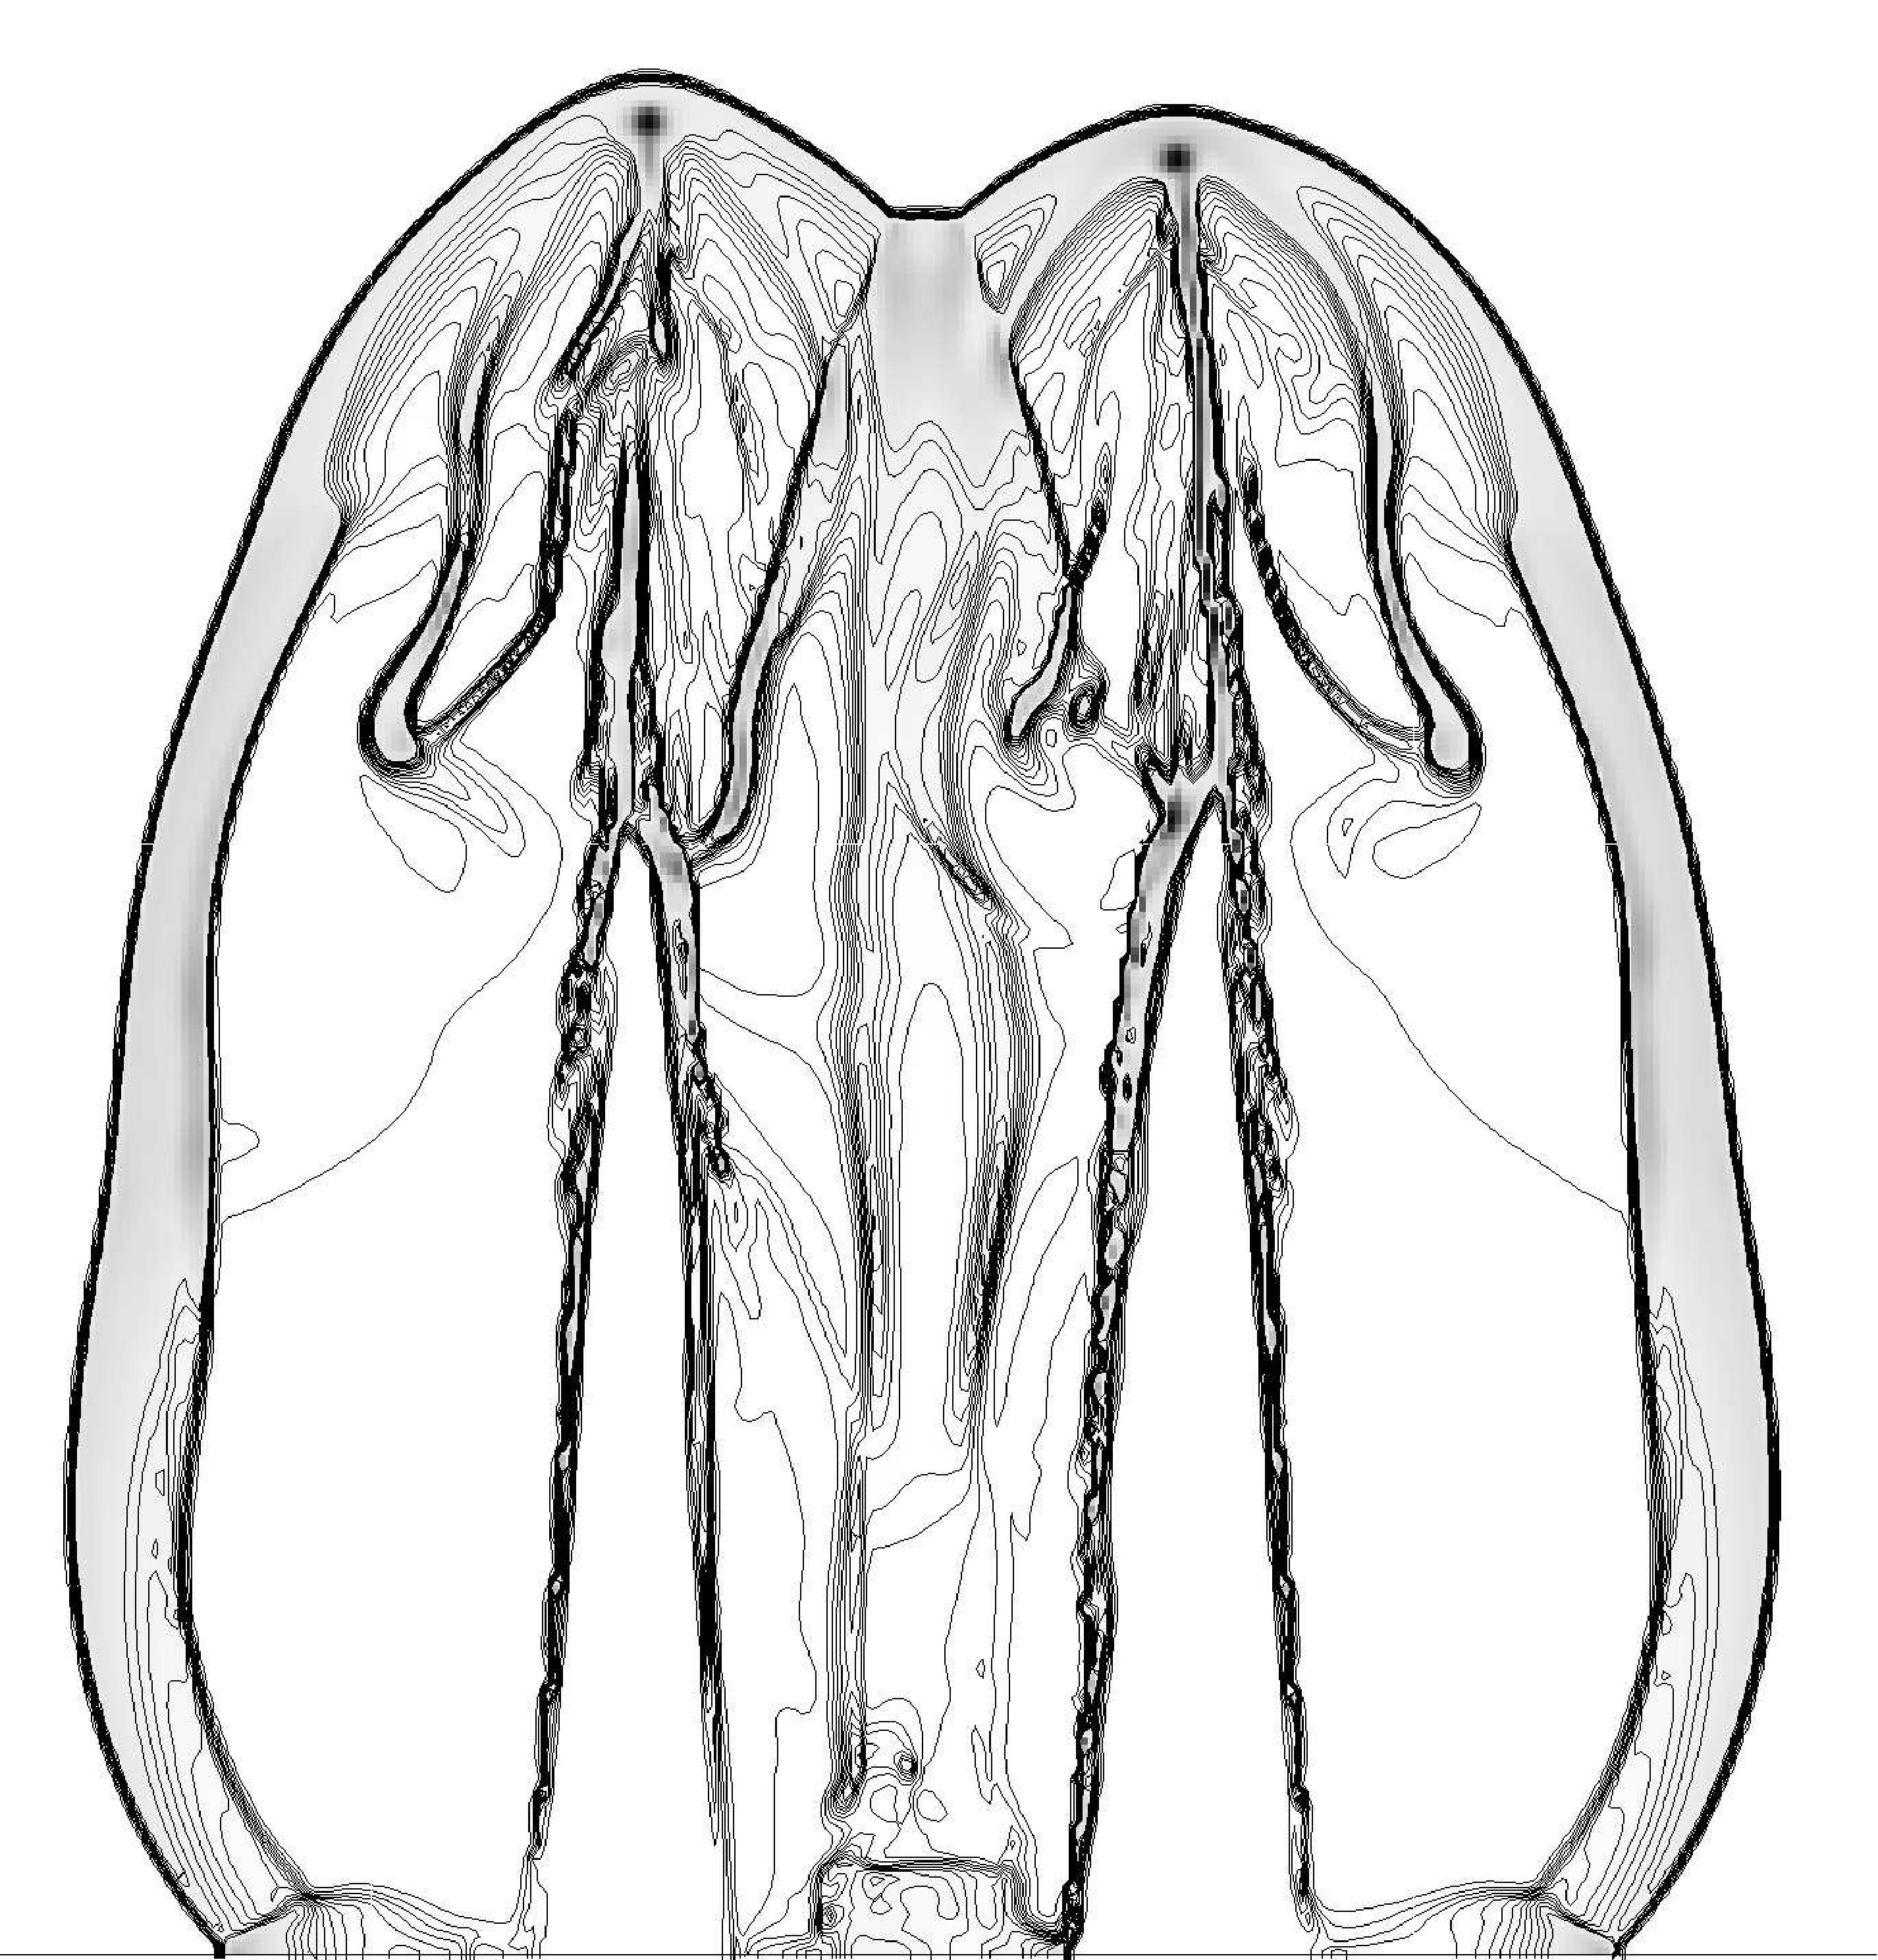
\includegraphics[width=8cm]{twinjet1}
%\caption{Computed isopycnics for $300\mathrm{km}s^{-1}$ twin jets at $t$=187 years }
%\label{fig:3} % Give a unique label
%\end{figure}

\section{Numerical constraints}

%There are several requirements on a code to perform MHD jet simulations.
% There are a large number of numerical schemes for solving the MHD equations
% However this system has several problem-specific peculiarities.
There are several constraints imposed on any numerical scheme to produce meaningful physical results.
Any numerical scheme must be \emph {consistent} with the original differential equations.
It must \emph{converge} upon the analytical result.
It must \emph{conserve} energy, momentum and mass.
It must be \emph{accurate} to some predefined order of accuracy.
Finally the scheme must be \emph{stable}, meaning its numerical errors must be bounded for a fixed timestep.
The numerical constraints do not end here, however as
the simulation of large-scale multidimensional MHD shocked flows presents several more intricate numerical difficulties.
% Godunov
For shocked flow the scheme must also capture shocks correctly (i.e. estimate their speed correctly).
The scheme must be \emph{upwind}, by which it is meant that information does not propagate at an unphysical velocity.
% Constrained Transport
For magnetised flow it is necessary to explicitly forbid the numerical creation of magnetic monopoles.
(This is the well known constraint on the divergence of the magnetic field.)
% Subcycling
Modelling radiative cooling losses implies reducing the thermal pressure, which can sometimes result in an unphysical negative pressure, as well as a constraint on the timestep, since radiative cooling losses happen on a much shorter timescale than the dynamical timestep.
% Adaptive Mesh
In addition, since large scale, three-dimensional flows are in question, reproducing the physics at a required order of accuracy becomes more computationally intensive. One method for reducing the amount of computations is the use of adaptive mesh refinement.


%\begin{enumerate}
%%\item Consistency:
%A \emph{consistent} scheme is one whose discretised equations tend to the differential
%equations when $\Delta t$ and $\Delta x$ tend to zero. 
%\item Convergence: 
%A finite difference scheme approximating a partial differential equation is a
%\emph{convergent} scheme if for any solution to the PDE, u(x,t) with solution to the
%finite difference scheme $u_m$ such that $u_m$ converges to $u(x,0)$
%as $m*dx$ converges to x , then $u_m$ converges to $u(x,t)$
%as $(m*dx,n*dt)$
%converges to $(x,t)$ for $(dt,dx) \rightarrow (0,0)$
%\item Accurate
%Would like to have third order accuracy, dropping to second order in the
%region of shocks.
%\item Stability:
%Errors should remain uniformly bounded at fixed $\Delta t$
% \item Uphold the conservation laws
% Finite difference methods are based on the assumption that the initial
% conditions are continuous and differentiable. This is not true in the case of a
% discontinuity such as a shock wave, for example. Fortunately in the region of a
% shock wave one may use a weak solution of the system of equations which applies
% the Rankine-Hugoniot jump conditions across the shock. The weak solutions are
% not necessarily unique so an entropy condition is required which limits the
% choice of solution to the physically correct one. Also, the
% numerical flux function must be in conservation form i.e. it reduces to the true
% numerical flux for the case of constant flow.
% % why is upwinding important 
% \item Upwinded scheme -- a scheme does not take into account the direction
% in which information is travelling and therefore may include events which take
% place downstream of the propagating wave and which it should not know about.
% This can result in a solution that is not causal. An upwinded (donor-cell)
% method calculates the direction of each wave and ensures that only the correct
% waves are included.
% \item Resolve shocks correctly -- use a Riemann solver which approximates the solution.
% \item Preserve $\boldsymbol{\nabla} \cdot \mathbf{B} = 0$
% \item Resolve over a range of length scales -- rely on the adaptive mesh to do this.
% \item Include microphysics of radiative cooling -- without reducing the timestep significantly.
% \item Efficient use of resources
% \item Multidimensional scheme:
% CTU scheme includes transverse fluxes.
% \item Pass standard tests -- require confidence that the numerical code as
% implemented can satisfactorily reproduce 
% \item High-order scheme -- use 2nd and 3rd order algorithms.
% \end{enumerate}

\subsection{Shock-capturing Scheme}

%Shocks are the most important feature of astrophysical fluid dynamics -
%they appear in observations and in analytical models. 
The astrophysical shocks which manifest themselves in forbidden line emission
from optical jets are represented in numerical codes in the form of steep
discontinuities.
For a scheme with second-order accuracy in space, it is necessary to approximate the spatial derivative.
The discrete approximation will usually either overestimate or underestimate
the derivatives near discontinuities and this results in unphysical oscillatory
patterns somewhat like the Gibbs phenomenon.
These oscillations are further amplified on the next timestep (when the derivative is approximated again).
Therefore special care needs to be taken near discontinuous solutions.
%which can cause numerical algorithms to exhibit unphysical oscillations, which
%become amplified in time iterations.
Traditionally there are three methods for dealing with discontinuities which arise in finite difference schemes.
\begin{itemize}
\item Shock-smearing (Artificial Dissipation)
\item Linear hybrid schemes
\item Godunov's method
\end{itemize}

\subsection{Shock-smearing -- Artificial Dissipative Terms}
The addition of artificial dissipative terms was introduced in \citet{vonNeumann:1950:MNC}, in
order to ``give the shocks a thickness comparable to (but preferably somewhat larger than) the spacing of the points''. 
It models the high-order physical viscosity which causes real shocks to remain steep but smooth over a small distance.
However the physical viscosity is a great deal smaller than the artificial viscosity. 
(There is also a numerical viscosity, since the shock has some finite width thanks to the discrete sampling.)
This method has been superseded by more accurate representations of the shocks in the Godunov scheme. 
It results in unphysical smearing and lack of causality in a solution.
However artificial viscosity is still useful to smear the solution on the computational grid. 
% to deal with certain numerical instabilities (the Quirk instability) and also negative pressures.
%Balsara lists four good reasons to use artificial viscosity.
\citet{1998ApJS..116..133B} lists four good reasons to use (a small amount of) artificial viscosity.
These include:
\begin{itemize}
\item Smearing the small oscillations due to the presence of a grid with slow
strong shocks, as seen in \citet{1984jcp_colella_woodward}.
\item The Quirk instability -- observed when a strong shock is closely aligned to the grid, produces oscillations of the order of one grid cell perpendicular to the shock propagation direction.
\item Turbulence simulations -- where noise may affect short length scale structures.
\item Grid noise may prevent convergence on a solution when trying to iterate towards a steady state.
\end{itemize}


% The method has fallen into disfavour because it is not upwind
% it is not causal
% incorrect estimate of the shock speed.
% Artificial viscosity is still added to many schemes (including this one) in order to reduce unphysical oscillations.


\subsection{Linear hybrid schemes}
%Linear hybridisation joins a high order scheme (disadvantage: spurious oscillations) to a low order scheme (disadvantage: smooths discontinuities) to their mutual benefit. 
%Linear hybridised schemes are widely used eg TVD, FCT.
%WENO
The idea behind the hybrid scheme is to use a high-order method for smooth regions and a low order method near discontinuities. The two methods are used in a weighted combination where the weight is related to some measure of the variation in the field.
This method has been consistently improved from its early implementations.
The earliest implementation was in the Flux-corrected transport scheme \citep{BB73}.
This was later improved into the Total Variation Diminishing scheme \citep{1983JCoPh..49..151H}.
It was further improved to the Essentially Non-Oscillatory scheme \citep{HEOC:1987}, and the Weighted Essentially Non-Oscillatory \citep{1994JCoPh.115..200L}.




\subsection{Godunov's Method}

The numerical solution of problems involving discontinuities (shocks) is made
difficult by the tendencies of high-order schemes to produce spurious
oscillations in the region of shocks. In particular Godunov's theorem
\citep{Go59} states that for the linear advection equation there are no schemes
of second order accuracy which satisfy the monotonicity condition. Similarly
for first order schemes the tendency is to smear the shock wave across a number
of cells, attaining monotonicity at the expense of a less accurate reproduction
of the solution. 
\citep{Go59} exploited the existence of discontinuities in a very physically insightful way.
Godunov treated each cell interface as a Riemann
problem, where the left and right states are given by the averaged values of theadjacent cells.
cells.
The key advantage of the Godunov scheme over the other schemes is that is
upwind. The explicit computation of the direction of each wave guarantees that
no information will propagate backwards in time. The disadvantage of this is
that the computation is extremely expensive, far more than a simpler method
\citep[e.g.][]{LW60} would be.

\subsubsection{The Riemann Problem}

\begin{figure*}[t]
\centering
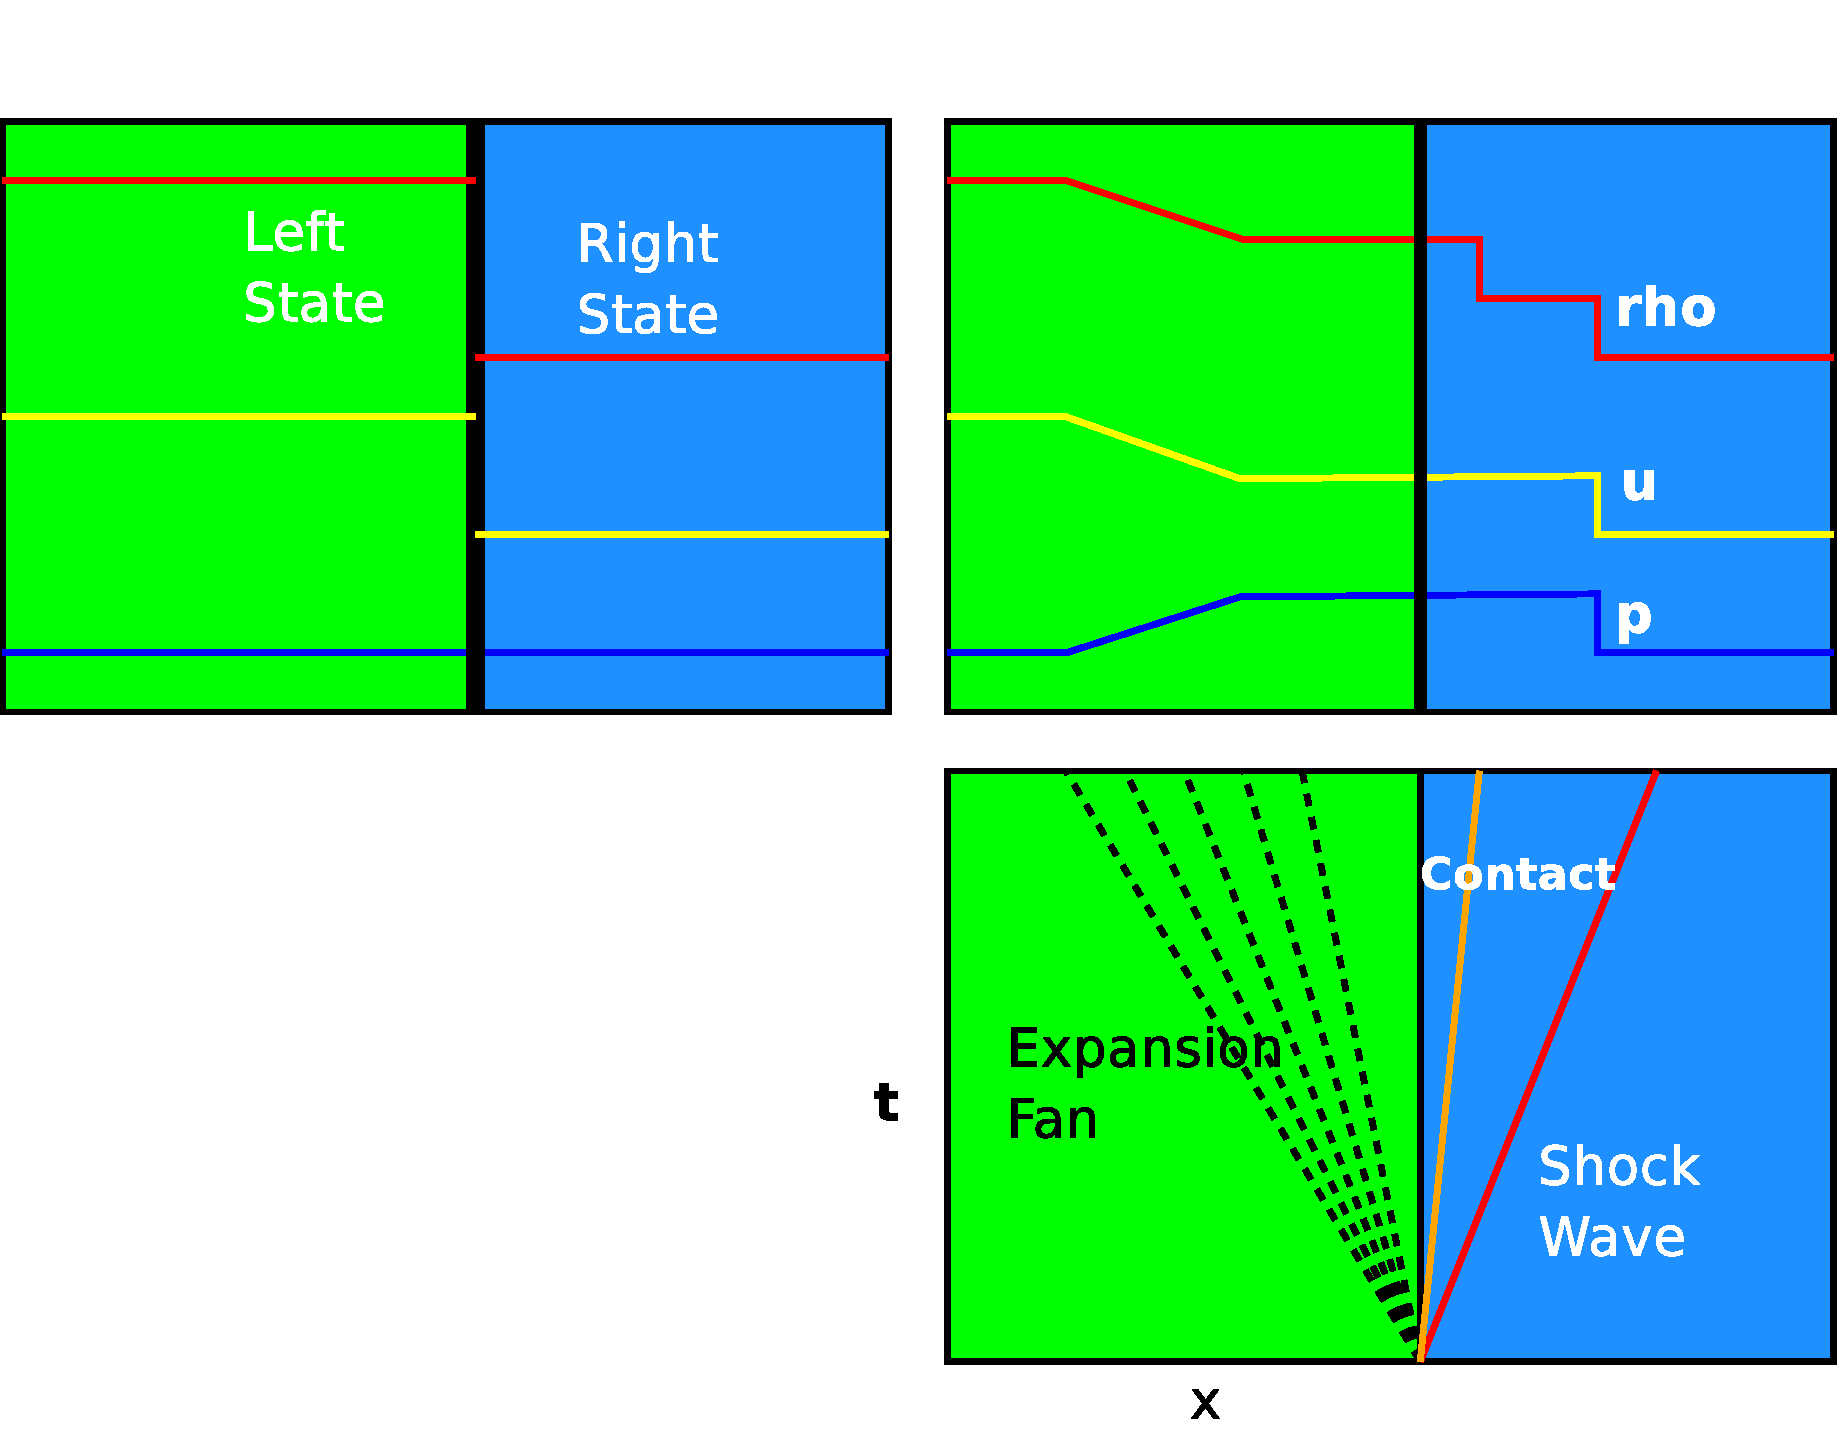
\includegraphics[width=\textwidth]{RiemannProblem}
\caption{
The top two panels show the initial and final states for a purely hydrodynamical one-dimensional shock tube problem. 
The lower right panel shows the $x$-$t$ characteristics for the same problem. 
(Figure from Haque 2006).
}
\label{fig:RiemannProblem} % Give a unique label
\end{figure*}

The Riemann problem is an initial value problem consisting of two states, ``left'' and ``right''
states separated by a discontinuity. Physically it may be pictured as a shock
tube, where two gases with different densities and pressures are separated in a
chamber by a thin membrane. At a time t, the membrane is removed. The subsequent
motion of the gases was calculated by Bernhard Riemann in 1859. The problem has
an exact analytical solution for the Euler and MHD equations for physically
meaningful input conditions, which may be discovered by calculating the
Rankine-Hugoniot jump conditions across the shock. This takes into account the
physical direction of propagation of information, thereby ensuring that the
solution uses only upwind information.

\begin{equation}
\begin{array}{c}
s [\rho]= [\rho u_x] \\
s [\rho u_x]= [\rho u^2 + P  -\frac{1}{2}{B_x}^2] \\
s [\rho u_y]= [ \rho u_x u_y - B_x B_y] \\
s [\rho u_z]= [\rho u_x u_z - B_x B_z] \\
s [B_y]= [u_x B_y - B_x u_y]\\
s [B_z]= [u_x B_z - B_x u_z]\\
s [E] = [ u_x \left( E + P\right) -B_x\left( \mathbf{v \cdot B} \right)]
\end{array}
\end{equation}
Rankine-Hugoniot Jump Conditions. s is the shock speed, $\rho$ is the density, $u_{x,y,z}$ the velocity components, $B_{x,y,z}$ the magnetic field, E the energy and P = $p_{thermal} + \frac{1}{2}\mathbf{B}^2 $ the total pressure.

\subsubsection{Exact Solution of the Riemann Problem}
The Godunov method requires that the fluxes across the boundaries be computed.
In the hydrodynamic case this can be done exactly.
An analytical solution of the nonlinear Riemann problem can be found by applying the Rankine-Hugoniot conditions across the shock.
The analytical solution of the MHD equations exists for the nonlinear Riemann problem.
The solution is implicit in five unknowns and requires an iterative method to compute the exact solution.
Solving the Riemann problem exactly in order to merely determine the fluxes is computationally expensive and wasteful, since the solution is only required at one region (the cell interface).
Exact iterative solutions to the Euler Riemann problem may be found in e.g. \citet{Toro:1997:RSN}.
Exact iterative solutions to the MHD Riemann problem have been computed by \citet{1988JCoPh..75..400B}, \citet{1998MNRAS.297..265F}.

\subsubsection{Linearised solution of the Riemann problem}
\citet{Roe81:_approx} proposed an alternative approach for the Euler equations.
To solve the system:
\begin{equation}
\frac{\partial \mathbf{U} }{\partial t}+
\frac{\partial \mathbf{F} }{\partial x}
+
\frac{\partial \mathbf{G} }{\partial y}
+
\frac{\partial \mathbf{H} }{\partial z}
=0
\end{equation}

where
$
\mathbf{U}=\left(
\rho , 
\rho u_x ,
\rho u_y  ,
\rho u_z  ,
E ,
B_x,
B_y  ,
B_z 
\right)
$
and 

%\begin{equation}
%\mathbf{U}=\left(
%\begin{array}{c}
%\rho  \\
%\rho u_x  \\
%\rho u_y   \\
%\rho u_z  \\
%E \\
%B_x
%B_y  \\
%B_z 
%\end{array}
%\right)
%\end{equation}

and the vectors $ \mathbf{F} , \mathbf{G}$ and $ \mathbf{H}$ are the y and z components of the flux.
\begin{equation}
\mathbf{F}=\left(
\begin{array}{c}
\rho u_x \\
\rho u_x u_x +p - B_x B_x  \\
\rho u_x u_y  - B_x B_y \\
\rho u_x u_z  - B_x B_z\\
(E+p)u_x - (\mathbf{u.B})B_x \\
0\\
B_y u_x - u_y B_x\\
B_z u_x -u_z B_x 
\end{array}
\right)
\end{equation}

\begin{equation}
\mathbf{G}=\left(
\begin{array}{c}
\rho u_y \\
\rho u_y u_x  - B_y B_x  \\
\rho u_y u_y +p - B_y B_y \\
\rho u_y u_z  - B_y B_z\\
(E+p)u_y - (\mathbf{u.B})B_y \\
B_x u_y -u_x B_y \\
0\\
B_z u_y -u_z B_y 
\end{array}
\right)
\end{equation}

\begin{equation}
\mathbf{H}=\left(
\begin{array}{c}
\rho u_z \\
\rho u_z u_x  - B_z B_x  \\
\rho u_z u_y  - B_z B_y \\
\rho u_z u_z +p - B_z B_z\\
(E+p)u_z - (\mathbf{u.B})B_z \\
 B_x u_z - u_x B_z \\
 B_y u_z - u_y B_z \\
0
\end{array}
\right)
\end{equation}

\begin{equation}
\frac{\partial \mathbf{U} }{\partial t}+
\frac{\partial \mathbf{F} }{\partial \mathbf{U}}
\frac{\partial \mathbf{U} }{\partial x}
+
\frac{\partial \mathbf{G} }{\partial \mathbf{U}}
\frac{\partial \mathbf{U} }{\partial y}
+
\frac{\partial \mathbf{H} }{\partial \mathbf{U}}
\frac{\partial \mathbf{U} }{\partial z}
=0
\end{equation}

Roe decided to linearise the system and solve the linearised version exactly.
The Jacobian matrices 
$\frac{\partial \mathbf{F} }{\partial \mathbf{U}}$,
$\frac{\partial \mathbf{G} }{\partial \mathbf{U}}$ and
$\frac{\partial \mathbf{H} }{\partial \mathbf{U}}$ 
are replaced by linearised matrices $ \mathbf{\tilde{A}}, \mathbf{\tilde{B}} , \mathbf{\tilde{C}}$ according to some averaging scheme.
\begin{equation}
\frac{\partial \mathbf{U} }{\partial t}+
\mathbf{\tilde{A}} \frac{\partial \mathbf{U} }{\partial x}
+\mathbf{\tilde{B}} \frac{\partial \mathbf{U} }{\partial y}
+\mathbf{\tilde{C}} \frac{\partial \mathbf{U} }{\partial z}
=0
\end{equation}
If this is accurate enough the exact solution to the nonlinear problem, with its attendant use of iterative solvers to find the roots of the implicit equation, is not required.
%First, the non-linear system was linearised using the method of Roe averages.
Although Roe chose an average which returned the exact solution for a shock, it
has been found that using the arithmetic average works just as well in many
cases.
Once this has been done the linearised system can be solved exactly.

The boundary state and therefore the flux on the boundary may be determined by adding the contributions from each linear wave.
This can be done in terms of the conserved or primitive fluxes or variables.
It is convenient to work in terms of the primitive variables, $\mathbf{P}$.

\begin{equation}
\mathbf{P}=\left(
\begin{array}{c}
\rho \\
u_x \\
u_y \\
u_z \\
p \\
B_x \\
B_y \\
B_z 
\end{array}
\right)
\end{equation}

\begin{equation}
\mathbf{P} =
\left\{
\begin{array}{c}
\mathbf{P_L} + \sum_{\lambda > 0} \left( \mathbf{l} \cdot\left( \mathbf{P_L -P_R} \right)\right)  \mathbf{ r}  \\
\mathbf{P_R} - \sum_{\lambda < 0} \left( \mathbf{l} \cdot\left( \mathbf{P_L -P_R} \right) \right)  \mathbf{ r} 
\end{array}
\right. 
\end{equation}
where $\mathbf{l,r}$ are the left and right eigenvectors of the linearised matrix,
and $\mathbf{P_L} , \mathbf{P_R} $ are the left and right states.
This works well in the strictly hyperbolic hydrodynamic case but caution must be exercised for the MHD equations.

\begin{equation}
\lambda=\left(
\begin{array}{c}
u-c_f \\
u-c_a \\
u-c_s \\
u \\
u+c_s \\
u+c_a \\
u+c_f 
\end{array}
\right)
\end{equation}

Unlike the HD equations, the MHD equations are not strictly hyperbolic \citep{1988JCoPh..75..400B}, at umbilic points their eigenvalues are not unique and the solution becomes singular or undefined.
In particular in the case when B$_x$=0 and when ${B_t}^2={B_y}^2 + {B_z}^2$=0 the eigenvalues may coincide.
When $|B_x|=0 $ the Alfv\'en speed $c_a = B_x / \sqrt{\rho}$ is zero, the slow speed collapses to zero and there is a double eigenvalue.
When $|B_t|$ is zero the fast speed collapses to the greater of the sound and Alfv\'en speeds and the slow speed collapses to the other.
When $|B_t|$ is zero and the Alfv\'en speed is equal to the sound speed (the magnetosonic or triple umbilic case) the fast, slow and Alfv\'en speeds all collapse onto the sound speed.
\citet{1988JCoPh..75..400B} found a linearisation for the case $\gamma = 2$.
\citet{Roe:1996:NEM} solved the system for an arbitrary value of $\gamma$.
\citet{1998MNRAS.297..265F} pointed out that ordinary gasdynamics may be used to solve at umbilic points.


\subsection{Reconstruction-Evolution Method}


\begin{figure*}[t]
\centering
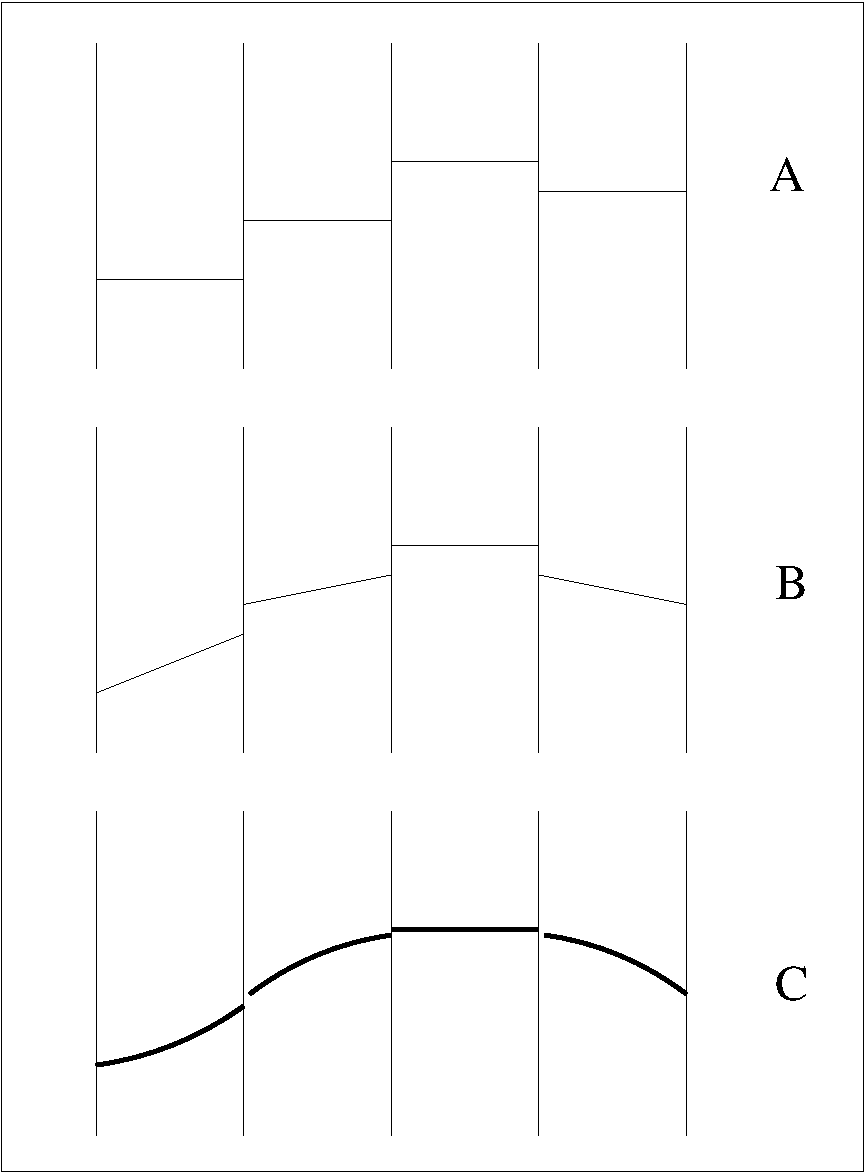
\includegraphics[width=8cm]{Reconstruction}
\caption{
Piecewise-constant, piecewise linear and piecewise parabolic reconstruction of the cell interface values.
}
\label{fig:Reconstruction} % Give a unique label
\end{figure*}


%The Piecewise Parabolic Method (PPM) \citep{1984jcp_colella_woodward} is the accurate high-resolution algorithm used by to perform time integration.
%It is based on the idea of Godunov that that a set of data points may be treated as a set of Riemann problems which need to be solved. The solution to the Riemann problem not only has an analytical solution, but also can be approximated by a linear solver -- which is even easier to solve without losing too much accuracy.
%There are several higher-order extensions of 
Godunov's original method uses the cell centred values as inputs to the Riemann problem. 
This loses a lot of information about the original cell structure. 
Van Leer attempted to recover some of this information by \emph{reconstructing} the cell as a linear function (using the neighbouring cell values). 
The problem with this is that it introduces new extrema into the solution, so the use of a limiter is required to remove any new extrema.
\citet{1984jcp_colella_woodward} added an extra order of accuracy by approximating the cell interfaces using parabola in the Piecewise Parabolic Method.
%The uniform states of Godunov's original (first order) method have been extended to second order using linear approximations (the Piecewise linear method) and third-order using quadratic approximations (PPM).
%The main distinguishing feature of PPM is its use of parabola. 
In PPM, instead of treating a data point as a constant value and having a piecewise constant function, it interpolates between the points using parabola. 
This gives a more accurate (third-order) description of a smooth gradient than a piecewise constant function (only first-order accurate).
It can be summarised in three main steps:
\begin{enumerate}
\item It takes an initial sample of the solution at a time t=0 and uses the sample points to reconstruct the left and right states using polynomial reconstruction. 
In the case of PPM the polynomials are quadratics, for the Piecewise Linear Method the polynomials are first order. 
%Analogously 
%Quadratic interpolation gives a better representation of the actual shape of the solution than a linear or piecewise constant interpolation.
\item The reconstructed left and right states are used as inputs to the Riemann solver, which gives the interface state at time t+dt. 
\item The interface states are conservatively differenced to find the average value at the cell centre at time t+dt.
\end{enumerate}
This method is particularly good in one dimension, but loses some of its effectiveness when applied to two are more dimensions, hence a multidimensional correction is applied.

\begin{figure*}[t]
\centering
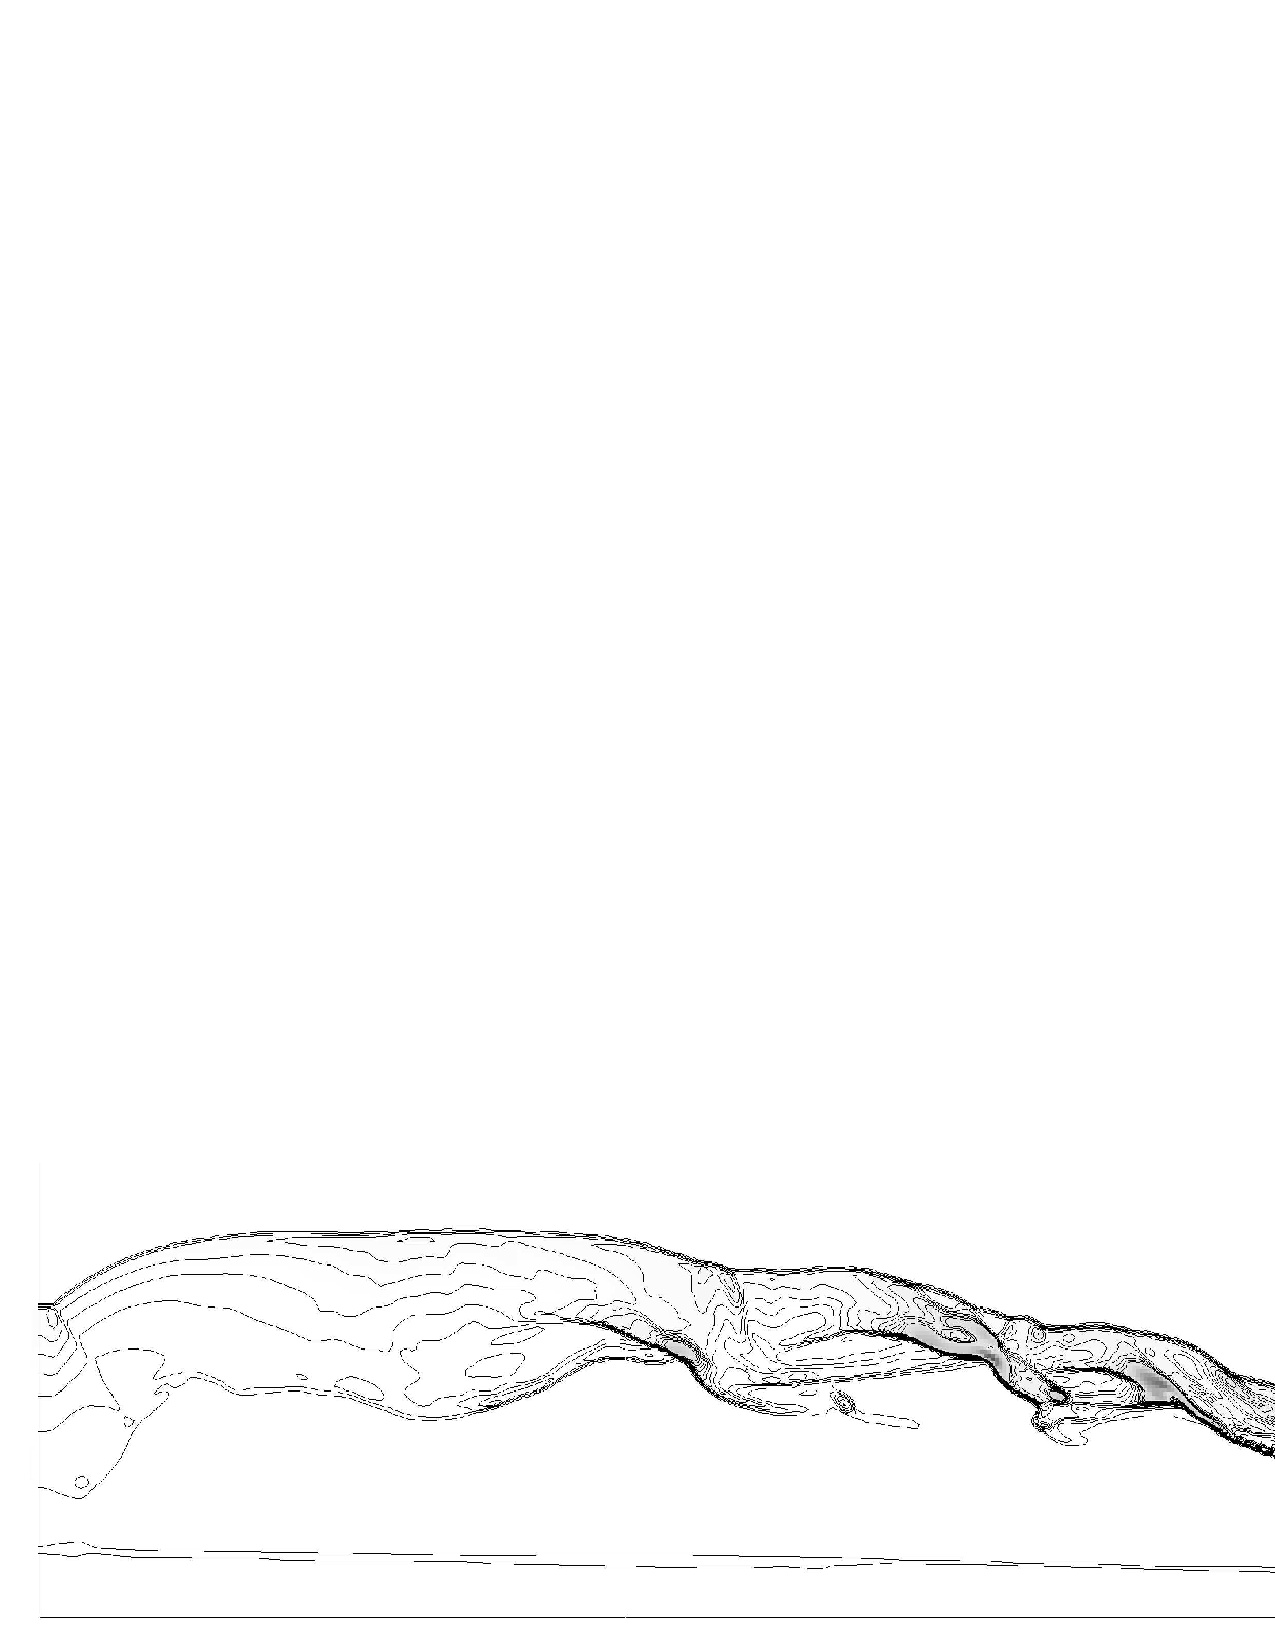
\includegraphics[width=15cm]{cooling}
\caption{
Isopycnics for 300~km~s$^{-1}$ purely hydrodynamic jet with atomic radiative cooling at $t=317$ years.
The adiabatic atomic jet has a bow shock which has been broken up by cooling -- causing loss of pressure which erodes the bow shape. 
}
\label{fig:2-1} % Give a unique label
\end{figure*}




\subsection{Multidimensional correction: The Corner Transport Upwind method}
\label{Multidimensional}
\subsubsection{Operator Split Method: Strang splitting}
% The Riemann solver approach does not work for 2D and higher
% The Riemann problem only has an analytical solution in 1D
% Extending the solver to 2D requires great care.
% Can use operator-splitting
% Strang splitting
The application of the inherently one-dimensional Riemann solver to a 2 or
more dimensional domain leads to the checkerboard instability,  where cells
become decoupled after the pattern of a chess or checkerboard. 
% Why? Because the physical wave is travelling at an angle to the grid.
There are two main approaches to including directional properties -- operator split and unsplit schemes.
An operator split scheme solves in each direction sequentially. 
Such a scheme needs to permute the sequence of directions after every timestep to get rid of a
directional bias. In 2D dimensions the solver permutes, x-y, y-x, x-y. In 3D this
becomes x-y-z, z-x-y, y-x-z etc. 
These alternating direction integration schemes are efficient, but because they are directionally operator-split it becomes difficult to enforce a divergence-free magnetic field. This is the major reason for using unsplit schemes.
\citep{Strang:1968:CCD}.

\subsubsection{Second Order Runge-Kutta }



In order to
correct for the extra dimension one must include the effects of the diagonal
cells. For example, by taking a halfstep in time and working out the fluxes we
indirectly include the effects of the diagonal cells which improves the
directional properties. This is the Runge-Kutta second order in time scheme. It can be straightforwardly extended to higher order methods.

This method has good directional properties but is merely a composite scheme. 
It does not explicitly compute the flux contributions travelling at an angle to
the grid. The method shows stability problems which become more limiting as the number of
dimensions is increased (going from 1D to 2D the maximum stable timestep is
decreased by one half and to 3D, by one third.
The CFL number is inversely proportional to the dimensionality (can be shown by Von Neumann stability analysis).
%Mignone says square root of dimensionality.
% But CTU is better. Why?

The stability problem is rooted in the fact that the numerical domain does not contain the true domain of dependence of the partial differential equation. 
Waves from the corner cells (see Figure \ref{fig:CTUMethod}) are not being included in the solution.
In particular the cross-derivative terms ($q_{yx}$ and $q_{xy}$) in the Taylor series expansion are ignored.

\begin{equation}
q(x,y,t_{n+1}) = q(x,y,t_n) + u \Delta t q_x - v \Delta t q_y
+ \frac{1}{2} (\Delta t)^2 \left[  
u^2 q_{xx} +
u v q_{yx} +
u v q_{xy} +
v^2 q_{yy} 
\right] 
+ \mathcal{O}( (\Delta t)^3 ) 
\end{equation}

\subsubsection{The Corner Transport Upstream Method}


\begin{figure*}[t]
\centering
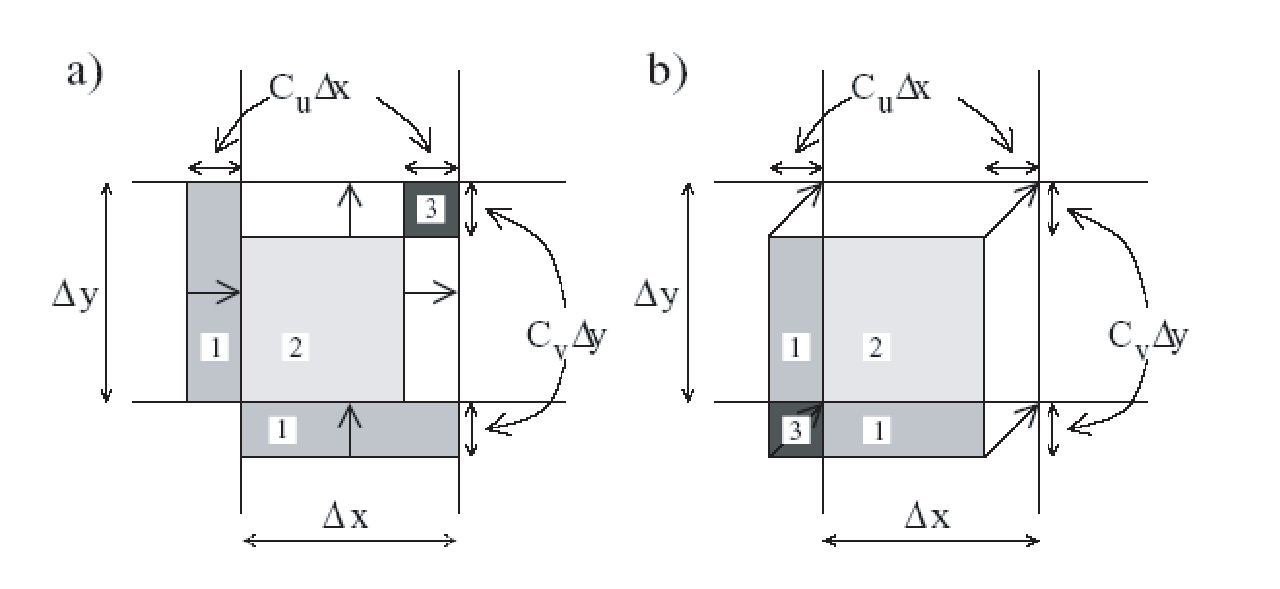
\includegraphics[width=9cm]{ctu}
\caption{
A depiction of the corner transport upwind method for the advection equation in two dimensions.
Using the method shown in the left panel results in the south west cell being unrepresented in the flow.
}
\label{fig:CTUMethod} % Give a unique label
\end{figure*}

To redress this shortcoming, several methods have been developed including the
Weighted Average Flux scheme of \citet{Toro:1997:RSN}, 
the Corner Transport Upwind (CTU) scheme due to \citet{Colella90:_multida} and 
the Method of Wave Propagation due to \citet{Leveque1997}. These three methods
possess a single goal, to compute a properly upwinded flux in more than one dimension.
% Colella set up values then solve Riemann problem
% Leveque solve Riemann 1st then distribute
% See MArti Muller Numerical Hydrodynamics in Special Relativity 
% http://www.livingreviews.org/lrr-2003-7  

% It's more expensive
%The CTU method uses a single step with multidimensional accuracy.


% How it works
In higher-order Godunov methods -- it is customary to construct a high-order approximation to the cell interface values to be used as inputs to the Riemann problem.
The CTU method is no different, and constructs a second-order approximation to the half-state as 

\begin{eqnarray}
U_{i+\frac{1}{2}}^{n+\frac{1}{2}} & = &
U_{i}^{n} \pm
\frac{\Delta x}{2} \frac{\partial \mathbf{U}}{\partial x}
+
\frac{\Delta t}{2} \frac{\partial \mathbf{U}}{\partial t} \nonumber\\
&= & 
U_{i}^{n} \pm
\frac{\Delta x}{2} \frac{\partial \mathbf{U}}{\partial x}
-
\frac{\Delta t}{2}
\left(
 \frac{\partial \mathbf{F}}{\partial x}
+ \frac{\partial \mathbf{G}}{\partial y}
\right) \\
&=&
U_{i}^{n} +
\left(
\pm
\frac{\Delta x}{2}
-
\frac{\Delta t A}{2}
\right)
\frac{\partial \mathbf{U}}{\partial x}
-
\frac{\Delta t}{2}
 \frac{\partial \mathbf{G}}{\partial y}
\nonumber
\end{eqnarray}

It can be seen that in the approximation to the interface state has a contribution from both the x and y directions.
The spatial derivative of the conserved flux, 
$ \frac{\partial \mathbf{U}}{\partial x}$,
may be approximated using either a central difference or a characteristic tracing.
The transverse flux correction,
$ \frac{\partial \mathbf{G}}{\partial y}$,
is computed using a Riemann solver.
The transverse flux correction correspond to the contribution from the corner cells in Figure \ref{fig:CTUMethod}.

%Since we  already have a method for finding $ \frac{\partial \mathbf{U}}{\partial t} $, the only unknown is $ \frac{\partial \mathbf{U}}{\partial x}$ , the spatial derivative of the conserved variables.

The corner transport upwind method has four steps.

\begin{enumerate}
\item Calculate approximations to the spatial derivative of the conserved variables,  $ \frac{\partial \mathbf{U} } {\partial x}$.
\item Construct left and right states at cell interfaces.
\item Solve the Riemann problem at cell interfaces.
\item Compute the time-updated state by straightforward conservative differencing.
\end{enumerate}


%It computes transverse fluxes from corner cells which are added on as corrections to the x-,y- and z-directional fluxes. By this means waves travelling at oblique angles are computed correctly.
% It ``preserves symmetries'' better
The CTU method has better stability properties than the Runge-Kutta method.
However it does come at a price, it computes many more Riemann problems per
timestep than other methods. Each cell face requires four Riemann solves in 3D so twelve in total per cell. For an operator split-scheme only three Riemann solves per cell are required.

% Artificial viscosity may be necessary to avoid certain numerical oscillations that occur when a oblique shock wave propagates closely aligned to the grid. The shock is smeared by a few cells using the method of \citet{Lapidus67}. This degrades the quality of the solution somewhat and is not necessary in all cases.  See Quirk instability and Sutherland (Local Oscillation Filter) paper.  See PPM paper and Colella-Woodward artificial viscosity, Falle viscosity, Balsara hyperviscosity.


\subsection{Satisfying and maintaining $\boldsymbol{\nabla} \cdot \mathbf{B} = 0$}


\begin{figure*}[t]
\centering
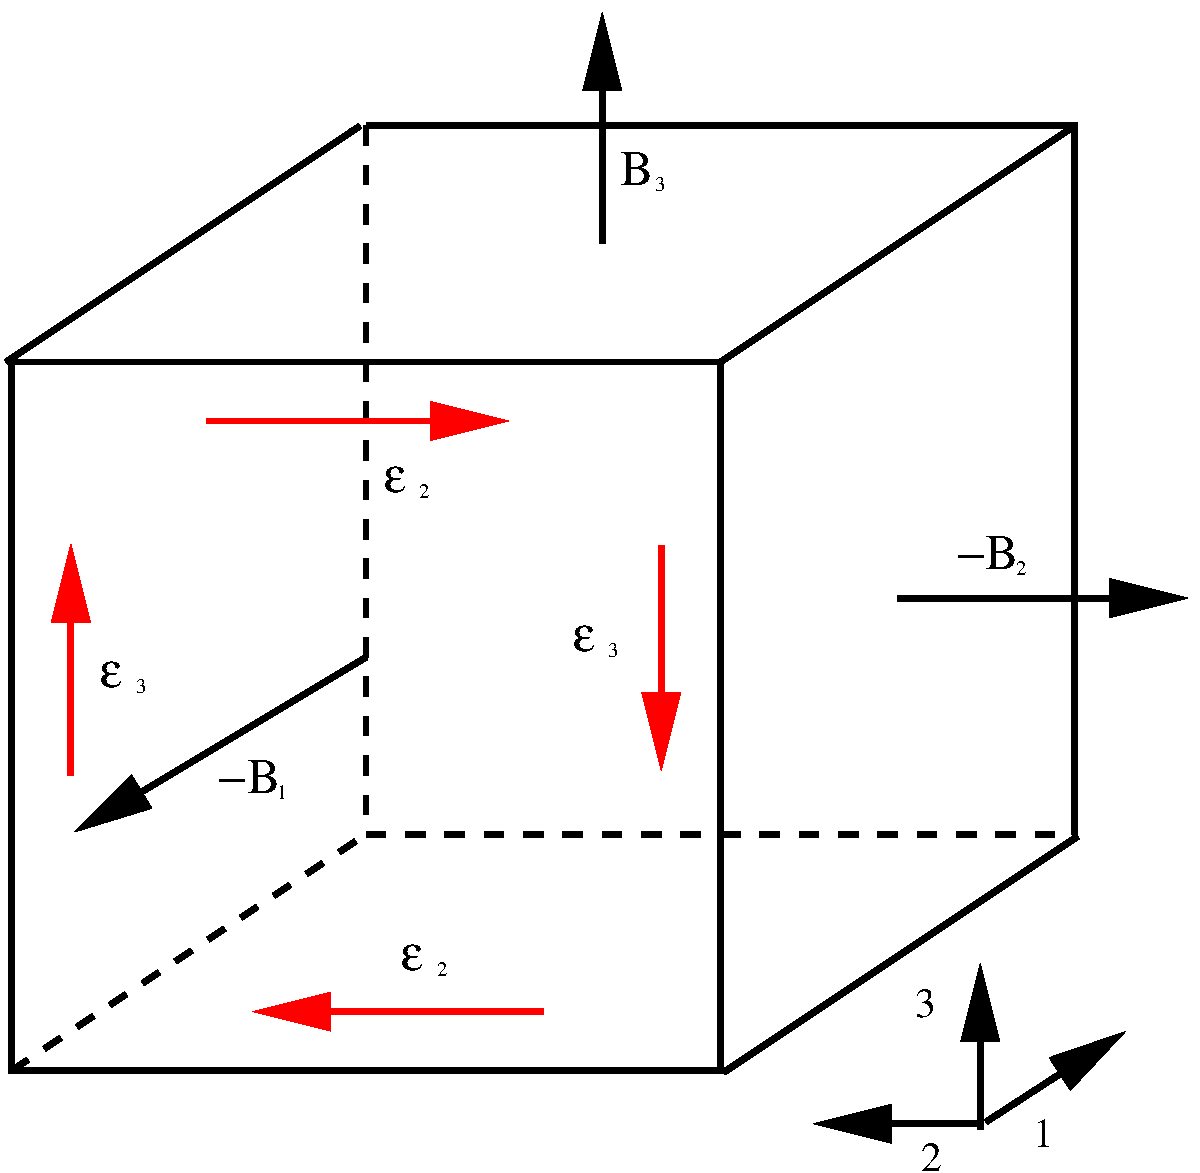
\includegraphics[width=9cm]{constraint_equation}
\caption{
The constrained transport method relies on the explicit use of Stokes' theorem, (Faraday's law), taking the path integral of the electric field, $\mathcal{E}$, around the closed contour, in this case the cell face shown by red arrows in the diagram.
}
\label{fig:2-21} % Give a unique label
\end{figure*}

% this is a big prob for MHD code since a small div b can cause a big mess

%In the course of the derivation of the MHD equations -- source terms appear which are proportional to $\boldsymbol{\nabla} \cdot \mathbf{B} $. 
The MHD equations include $\boldsymbol{\nabla} \cdot \mathbf{B} $ in their source terms.
As these terms are analytically zero they are often omitted from the
computation. Numerically, however, the field may be divergent and monopoles appear in the solution if the constraint equation is not explicitly imposed.
One of the most challenging problems for an MHD code is the preservation of $\boldsymbol{\nabla} \cdot \mathbf{B} =0$, which if not strictly maintained to machine accuracy can generate unphysical extra forces.
There are four different approaches: advecting the magnetic vector potential, using a staggered mesh, Hodge projection method (and a Poisson solver), or the Powell method, which consists of adding an eighth wave to advect $\boldsymbol{\nabla} \cdot \mathbf{B}=0$.
All these methods have advantages and disadvantages.
Advecting the magnetic vector potential is not useful in this context as it is not a conserved quantity and cannot be used for example with a Riemann solver.
In addition it requires an extra spatial derivative (to compute $\mathbf{B}=\nabla \times \mathbf{A} $) reducing the order of accuracy of the solution by at least one.
% Powell
The \citet{1999JCoPh.154..284P} method is based on idea of \citet{Go75} to convert the non-strictly hyperbolic MHD system to strict hyperbolicity using the concept of an imaginary eighth wave which advects the quantity $\boldsymbol{\nabla} \cdot \mathbf{B} $ at the velocity of the flow. 
The idea is that monopoles of positive and negative values are created in equal quantities and annihilate each other. 
%Dedner 
\citet{2002JCoPh.175..645D} extends this scheme to advect the $\boldsymbol{\nabla} \cdot \mathbf{B}$ wave at the fast magnetosonic velocity, i.e. the fastest velocity available.
The Poisson solver method simply computes a pseudo-potential ``correcting scalar field'' and subtracts the gradient of this field from the offending magnetic field components. 
This also produces a divergence free magnetic field.
It is computationally expensive.
The most elegant solution is the explicit use of Stokes' theorem to constrain the $\boldsymbol{\nabla} \cdot \mathbf{B}$ to machine accuracy.
$\boldsymbol{\nabla} \cdot \mathbf{B}=0$ is preserved using a staggered mesh algorithm \citep{307327}. 

The divergence-free constraint is enforced by using a difference form of Stokes' theorem to advect the field:
\begin{equation}
\frac{\partial \phi_S}{\partial t}= 
\int_{\partial S}  \mathbf{v} \times \mathbf{B} \cdot \mathbf{dl}
=\int_{\partial S}  \mathcal{E} \cdot \mathbf{dl}
\end{equation}
In difference form the equation is
\begin{eqnarray}
   \frac{\partial \Phi}{\partial t} &=&
	  - \mathcal{E}_{y,i,j} \delta y
	    - \mathcal{E}_{z,i,j} \delta z
		   + \mathcal{E}_{y,i,j} \delta y
			  + \mathcal{E}_{z,i,j+1} \delta z \\
   \frac{\delta \Phi_x}{\delta t} &=&
	  - \mathcal{E}_{z,i,j} \delta z
	    + \mathcal{E}_{z,i,j+1} \delta z \\
\frac{\delta \Phi_y}{\delta t} &=&
	+ \mathcal{E}_{z,i,j} \delta z
	- \mathcal{E}_{z,i+1,j} \delta z \\
   \frac{\delta \Phi'_x}{\delta t} &=&
  + \mathcal{E}_{z,i+1,j+1} \delta z
  - \mathcal{E}_{z,i,j+1} \delta z \\
   \frac{\delta \Phi'_y}{\delta t} &=&
  - \mathcal{E}_{z,i+1,j+1} \delta z
  + \mathcal{E}_{z,i+1,j} \delta z
\end{eqnarray}
The expressions for $\frac{\delta \Phi'_x}{\delta t}$ , $  \frac{\delta \Phi'_y}{\delta t}$, 
$ \frac{\delta \Phi_x}{\delta t} $
and $ \frac{\delta \Phi_y}{\delta t}$  all
sum to zero, indicating that the total flux is conserved over time.
The above equations when divided by area give an advection scheme for the flux density which preserves the divergence free condition.
%The magnetic field is computed at cell faces centres by integrating the electromotive force in a closed loop about each face. 
%The face-centred field is then projected back to the cell centre using an arithmetic average using a switch which detects the presence of a strong shock. 
This guarantees that the \emph{time changes} in the flux will be numerically divergence-free.

In order to ensure that the initial field is non-divergent, $\mathbf{B}$, the magnetic field strength is computed from the curl of the magnetic vector potential $\mathbf{A}$, by definition $\mathbf{B} = \mathbf{\boldsymbol{\nabla}} \times \mathbf{A}$, which has no divergence by the vector identity $ \boldsymbol{\nabla} \cdot (\boldsymbol{\nabla} \times \mathbf{A}) = 0$.


\subsection{Modelling the Microphysics of Atomic Radiative Cooling}
\label{ModellingtheMicrophysicsofAtomicRadiativeCooling}

% Raga cooling -- history of cooling 
%It is essential to include the microphysics of radiative cooling to model phenomena whose visibility depends on the loss of energy in the form of detectable radiation. 
% haven't done molecular cooling, but should really
% It might be okay for jets but not so good for molecular outflows
%Atomic cooling is used as in the temperature ranges $10^4 - 10^6$K atomic cooling dominates molecular cooling since the overwhelming majority of molecules dissociate at these temperatures.
%For lower-temperature molecular outflows this assumption would obviously not be valid.
%Modelling each electron collision is out of the question however as it would require resolution from the the typical length scale of interest 10$^{15}$ cm to the picometre scale, some 27 orders of magnitude. As a compromise a cooling function is used which represents on a macroscopic scale the rate of energy loss at this temperature range for a sample (solar) set of abundances.
%In addition to the conserved quantities the microphysics of energy lost due to radiative cooling ($L_{cooling}$) is represented using a cooling function adapted from \citet{1993ApJS...88..253S}. \citet{1993ApJS...88..253S} include the effects of electron collision ionisation, radiative and dielectronic recombination and line radiation within their cooling function.



Protostellar jets are strongly cooled by optically thin radiation emitted in the high-temperature post-shock regions.
%It is this emission which renders the objects visible.
Calculating radiative electron transitions directly is not feasible in the fluid approximation.
\citet{1997ApJS..109..517R} identify three commonly-used approximations to the inclusion of radiative effects:
\begin{enumerate}
\item Assume equilibrium \citep{1987ApJ...323..193R}
\item Non-equilibrium fully ionised \citep{1990ApJ...360..370B}
\item Non-equilibrium explicitly computed ionisation fraction \citep{1995MNRAS.272..785F}
\end{enumerate}
% use Falle and Raga
The third approach is used in the current work.
The ionisation equation is:
\begin{equation}
\frac{\partial \rho x_e}{\partial t} + \boldsymbol{\nabla} \cdot \left( \mathbf{v} \rho x_e \right)  = {\rho}^2 \frac{X_H}{m}\left[ x_e\left( 1-x_e  \right) \alpha \left( T \right) - {x_{e}}^2 \beta \left(  T \right) \right]
\end{equation}
where 
$x_e$ is the ionisation fraction,
$X_H$ is the hydrogen abundance,
m is the average particle mass,
$\alpha \left( T \right) $
and
$\beta \left( T \right) $
are the collisional ionisation and radiative recombination terms, and the other symbols have their usual meanings.
\begin{eqnarray}
\alpha \left( T \right)& =& K_I T^{\frac{1}{2}} exp \left( -1.579 \times 10^5 T\right) \\
\beta \left( T \right)& = & K_R T^{-0.7}
\end{eqnarray}
$K_I=6.417 \times 10^{-11}$ cm$^3$~s$^{-1}$~K$^{-1/2}$ and $K_R=2.871 \times 10^{-10}$ cm$^3$~s$^{-1}$~K$^{0.7}$ are the collisional ionisation and radiative recombination rate coefficients \citep{1995MNRAS.272..785F}. \footnote{Note that the recombination rate is incorrectly quoted in \citet{1995MNRAS.272..785F}. }

The microphysics of energy lost due to radiative cooling is represented using a
cooling function adapted from \citet{1993ApJS...88..253S} and depicted in Figure
\ref{fig:2-4}, which represents on a macroscopic scale the rate of energy loss at this temperature range for solar abundances.
\citet{1993ApJS...88..253S} include the effects of electron collisional ionisation, radiative and dielectronic recombination and line radiation within their cooling function.

\begin{figure}[t]
\centering
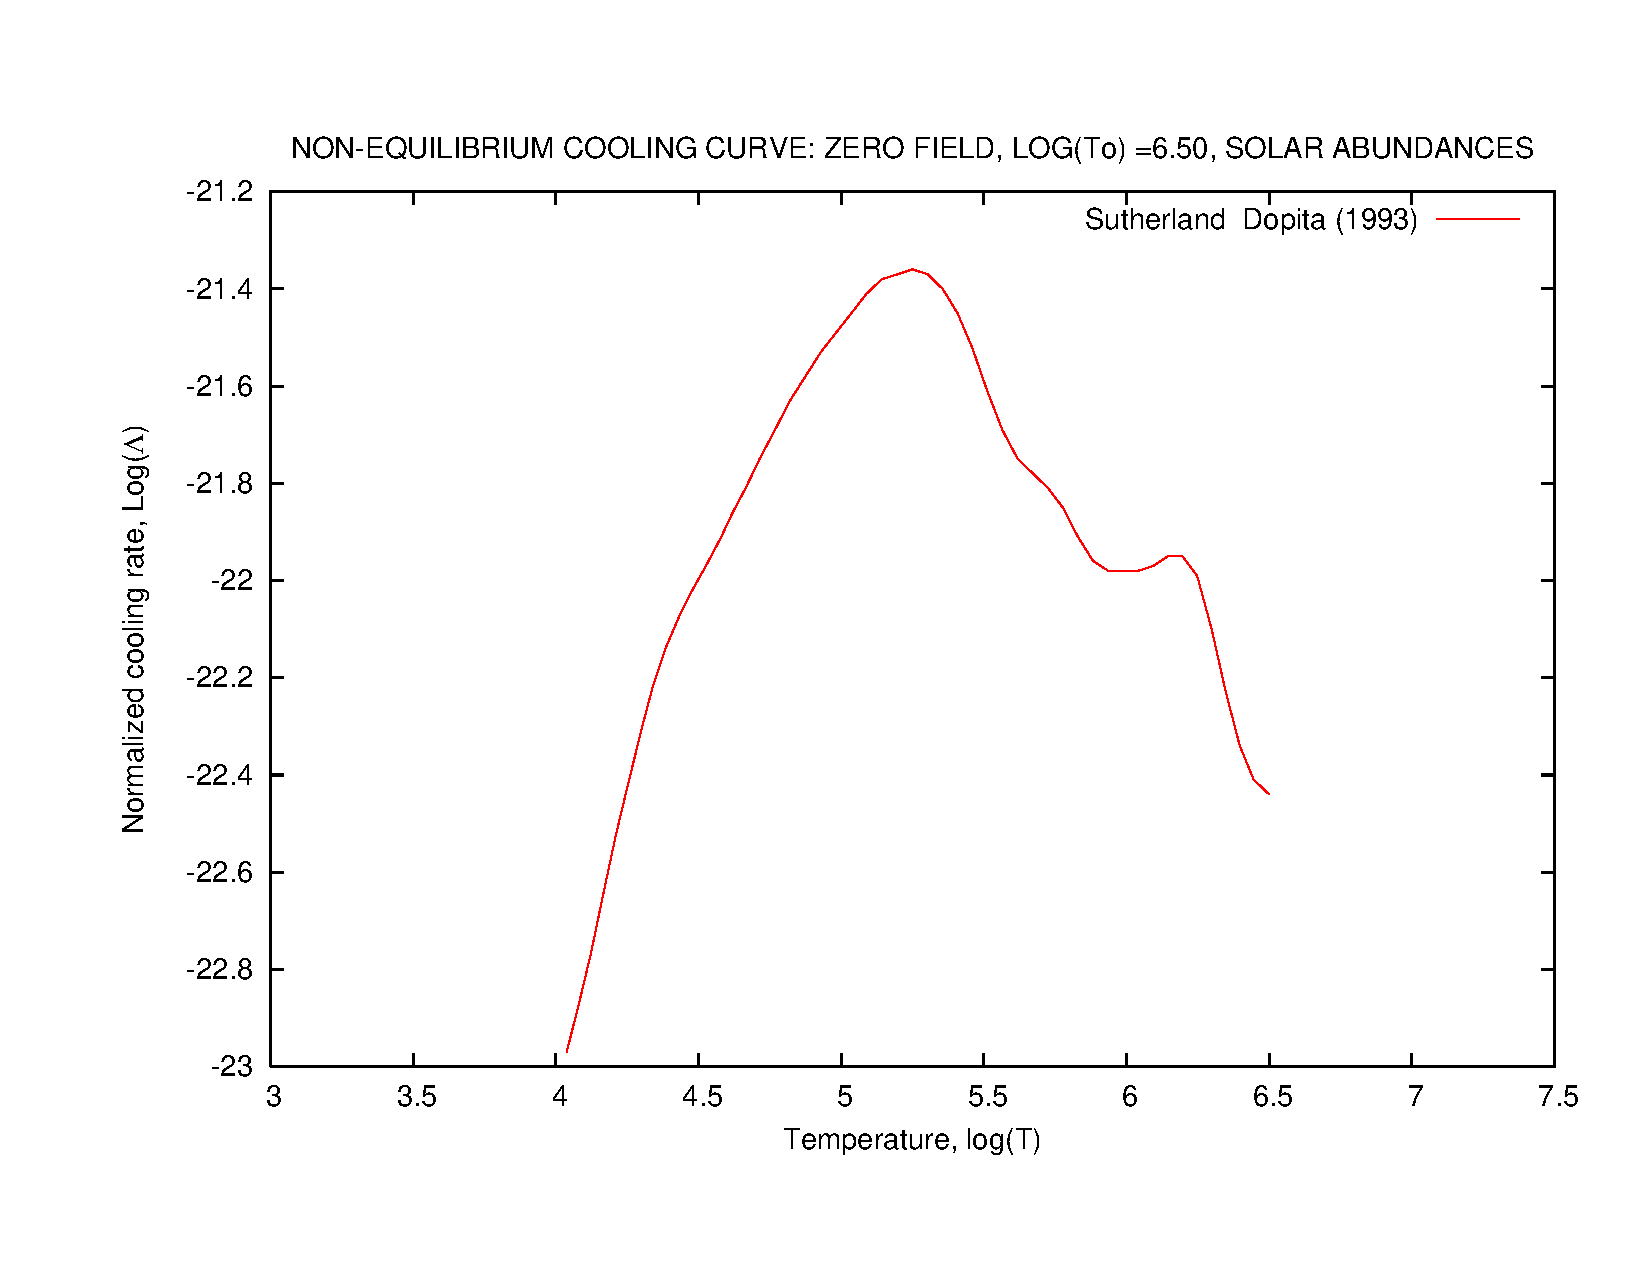
\includegraphics[angle=270,width=7cm]{sutherland}
\caption{
Log normalised radiative cooling loss $\Lambda$, where $L_{cooling}= \rho^2 \Lambda$ plotted against log temperature \citet{1993ApJS...88..253S}.
}
\label{fig:2-4} % Give a unique label
\end{figure}

Cooling models the physical process where energy is dissipated.
$L_{cooling}$ represents the cooling function in the conservation of energy equation.
\begin{eqnarray}
\frac{\partial E}{\partial t}
+\boldsymbol{\nabla}
\cdot
\left[
\left( E + p^*\right) \mathbf{u}
- (\mathbf{u}\cdot\mathbf{B})\mathbf{B}
\right] + L_{cooling} = 0
\end{eqnarray}
%In order to add cooling to the code need to subtract energy from the solution. 
As can be seen from Figure \ref{fig:2-4}, the loss of energy due to cooling depends on temperature in a highly non-linear fashion.
It represents several energy losing and gaining processes happening at atomic level in the fluid.
There is no simple mathematical function which can concisely represent these processes.
%It is therefore modelled using a cooling function from \citet{1993ApJS...88..253S} (Figure \ref{fig:2-4}). 

\begin{figure}[t]
\centering
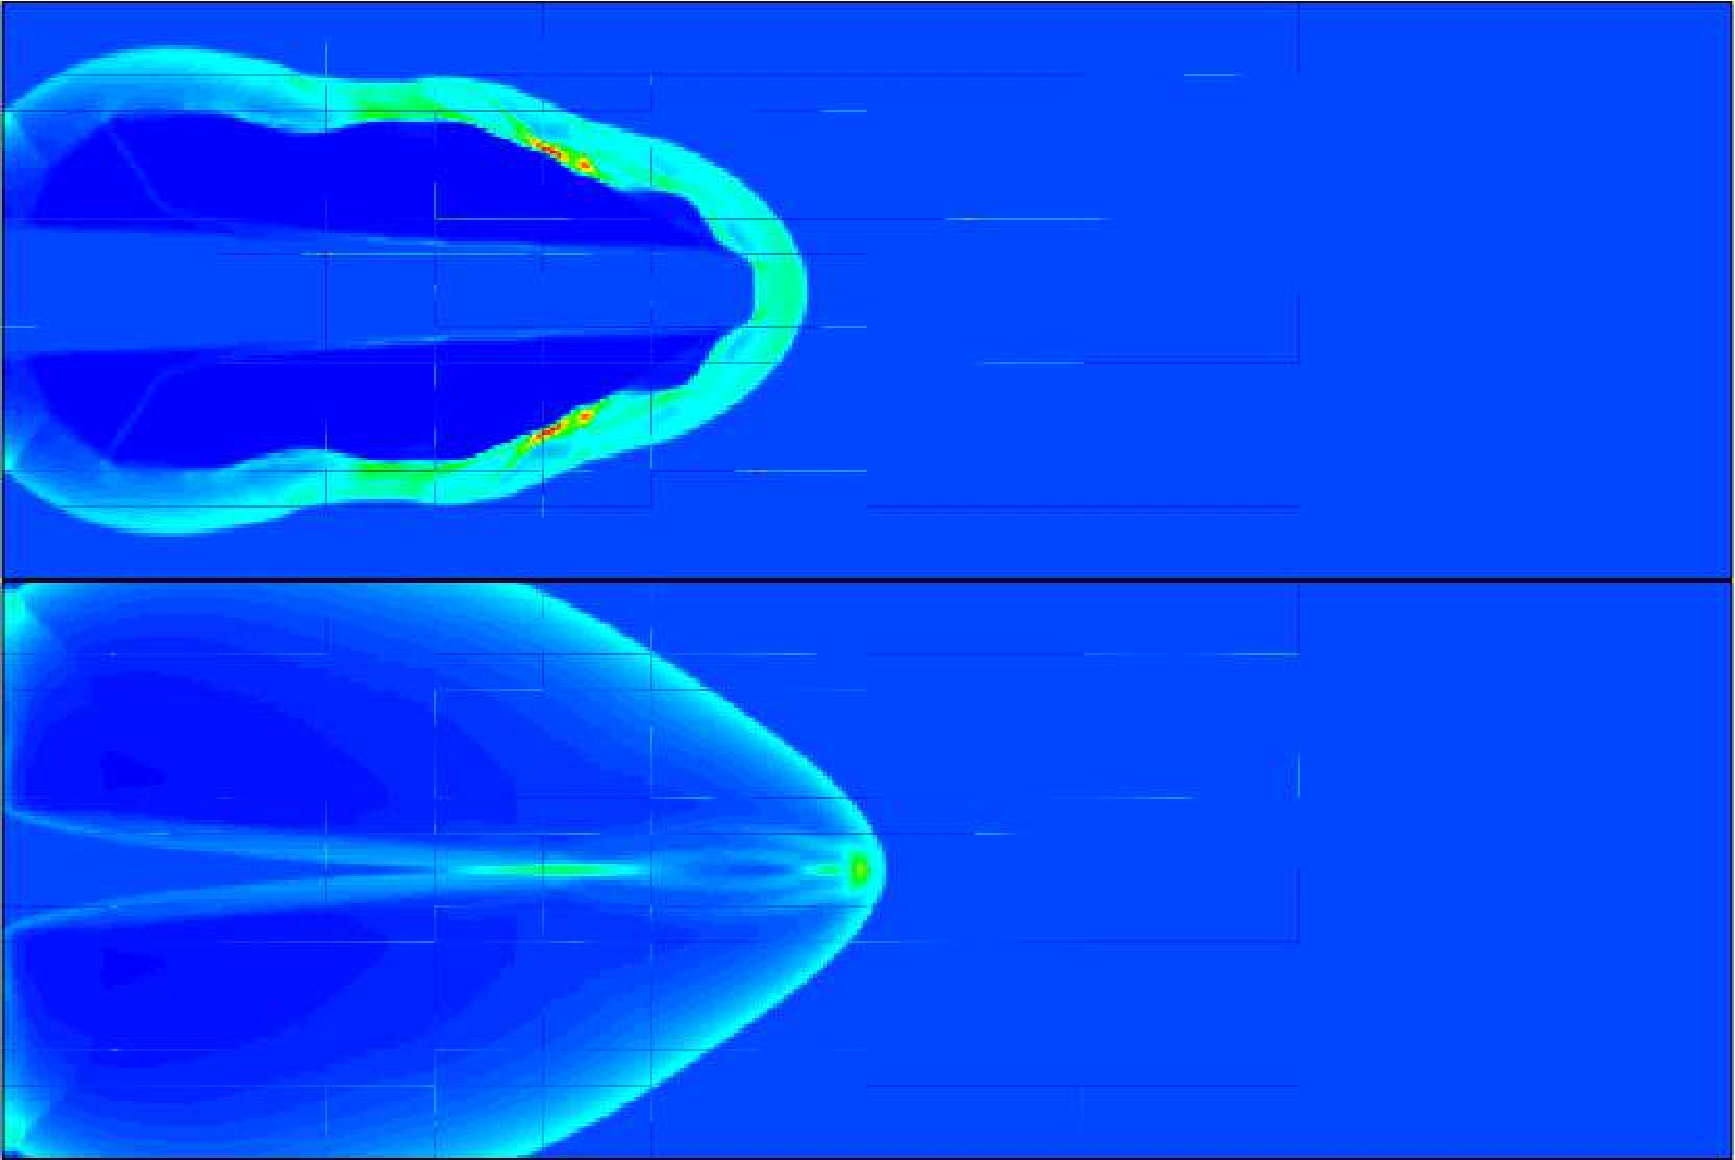
\includegraphics[width=7cm]{cool_compare}
\caption{
Density comparison of 2D slab-symmetric jet propagating with cooling turned off (lower panel) and on (upper panel).
Jet velocity = 300 km/s. Density, 120 cm$^{-3}$, temperature 1000 K.
The jets are density and pressure matched to the ambient medium. 
Note the slower speed of the cooled jet, the distortion of the bow shock, and the shape of the core of the jet.
}
\label{fig:2-5} % Give a unique label
\end{figure}

Figure \ref{fig:2-5} contrasts 2D slab-symmetric jets with and without atomic radiative cooling.
The jet morphology is entirely different; the cooled jet bow shock is much more irregular, as it has lost a lot of supporting thermal pressure.
The propagation velocity of the jet is also lowered (consistent with the jet
losing energy, \citet{1990ApJ...360..370B}).
% The importance of substepping

\begin{equation}
\frac{\partial E}{\partial t}
=
\frac{\partial F}{\partial x}
+
L_{cooling}
\end{equation}

%The cooling function gives a rate of energy loss versus temperature.
The cooling function tracks the rate of energy loss with temperature.
It is possible to simply calculate the temperature value at each timestep and read off the rate of energy loss from the look-up table.
However in general the cooling function is not smooth and in fact it changes quite rapidly.
The timestep if limited by the cooling will become quite short and the solution will become diffusive.
Since the cooling is localised at or near shocked regions the operator-split approach is extremely effective.

\begin{equation}
E^{t+dt}
=
E^t
+
\frac{\partial F}{\partial x} \Delta t
+
{\int_{t}}^{t+dt} L_{cooling}.dt
\end{equation}
%Subtracting a chunk of energy all at once during the course of a time step can cause the other variables not to have time to adjust their values -- so the energy is gradually removed during the time step in series of sub-cycles.


%\citet{1990ApJ...360..370B} derive a formula for the cooling length $d_{cool}$ of a jet in terms of its number density and bow shock velocity
%\begin{equation}
%d_{cool} = 4.5 \times 10^{-7} {n_0}^{-1} {v_{s,7}}^4 \mathrm{cm}
%\end{equation}

\section{An MHD 3D numerical code: ATLAS}
ATLAS is a new modular shock-capturing, multi-dimensional, staggered-mesh, adaptive-grid, directionally split, higher-order Godunov astrophysical MHD code, which uses a linearised Roe-type MHD Riemann solver.
It was written by Daniel S. Spicer and Stephen O'Sullivan at the NASA Goddard Space Flight Center.
ATLAS uses several leading alternative high-order Godunov schemes, including a
scheme, MUSCL \citep{1979JCP_vanLeer} modified to direct Eulerian form by
\citet{1984jcp_colella_woodward}, a second-order scheme, the piecewise linear
method (PLM) and a third-order scheme, the piecewise parabolic method
\citep[PPM;][]{1984jcp_colella_woodward}.
%The goal is to have a working MHD code that can demonstrably pass all the tests in the literature, to establish confidence in the results of its simulations.  Although computational methods for numerical solution of partial differential equations have been proposed as far back as \citet{1907PPSL...21...88R} -- it is only relatively recently that numerical codes have become essential to solve problems.  The numerical code must be able to handle shocks, preserve the conservation laws and maintain $\boldsymbol{\nabla} \cdot \mathbf{B} =0$.

\subsection{Parallelisation} 
ATLAS/PARAMESH uses the SPMD (Single Program Multiple Data) approach.
Each processor can access a copy of the same program but has its own separate data block to work on. 
Information at the boundaries of each block is stored in temporary guard/ghost cells. These represent an overhead in memory and CPU time.
PARAMESH takes care of most of the interprocessor communication, by dividing the data up into blocks organised into a hierarchical tree. 
The blocks are divided among the available processors using a Morton ordering scheme -- this ensures that neighbouring blocks are located on nearby processors. 
At every timestep, the blocks are redistributed among the processors which ensures that the load is efficiently balanced.
By adjusting the amount of blocks on each processor and the size of each block, a crude measure of control over the scaling of the problem may be obtained.
Simulations were carried out using the ATLAS code on a 64 node hyper-threaded ``Beowulf"-type cluster. (Theoretical peak performance 150 GHz.) The individual nodes on the cluster were 16 2.66 GHz dual processors with hyper-threading enabled -- a total of four processors, two real, two virtual. Shared memory was enabled on each node. 

\subsection{Achieving Higher Resolution using Adaptive Mesh Refinement}


\begin{figure}[t]
\centering
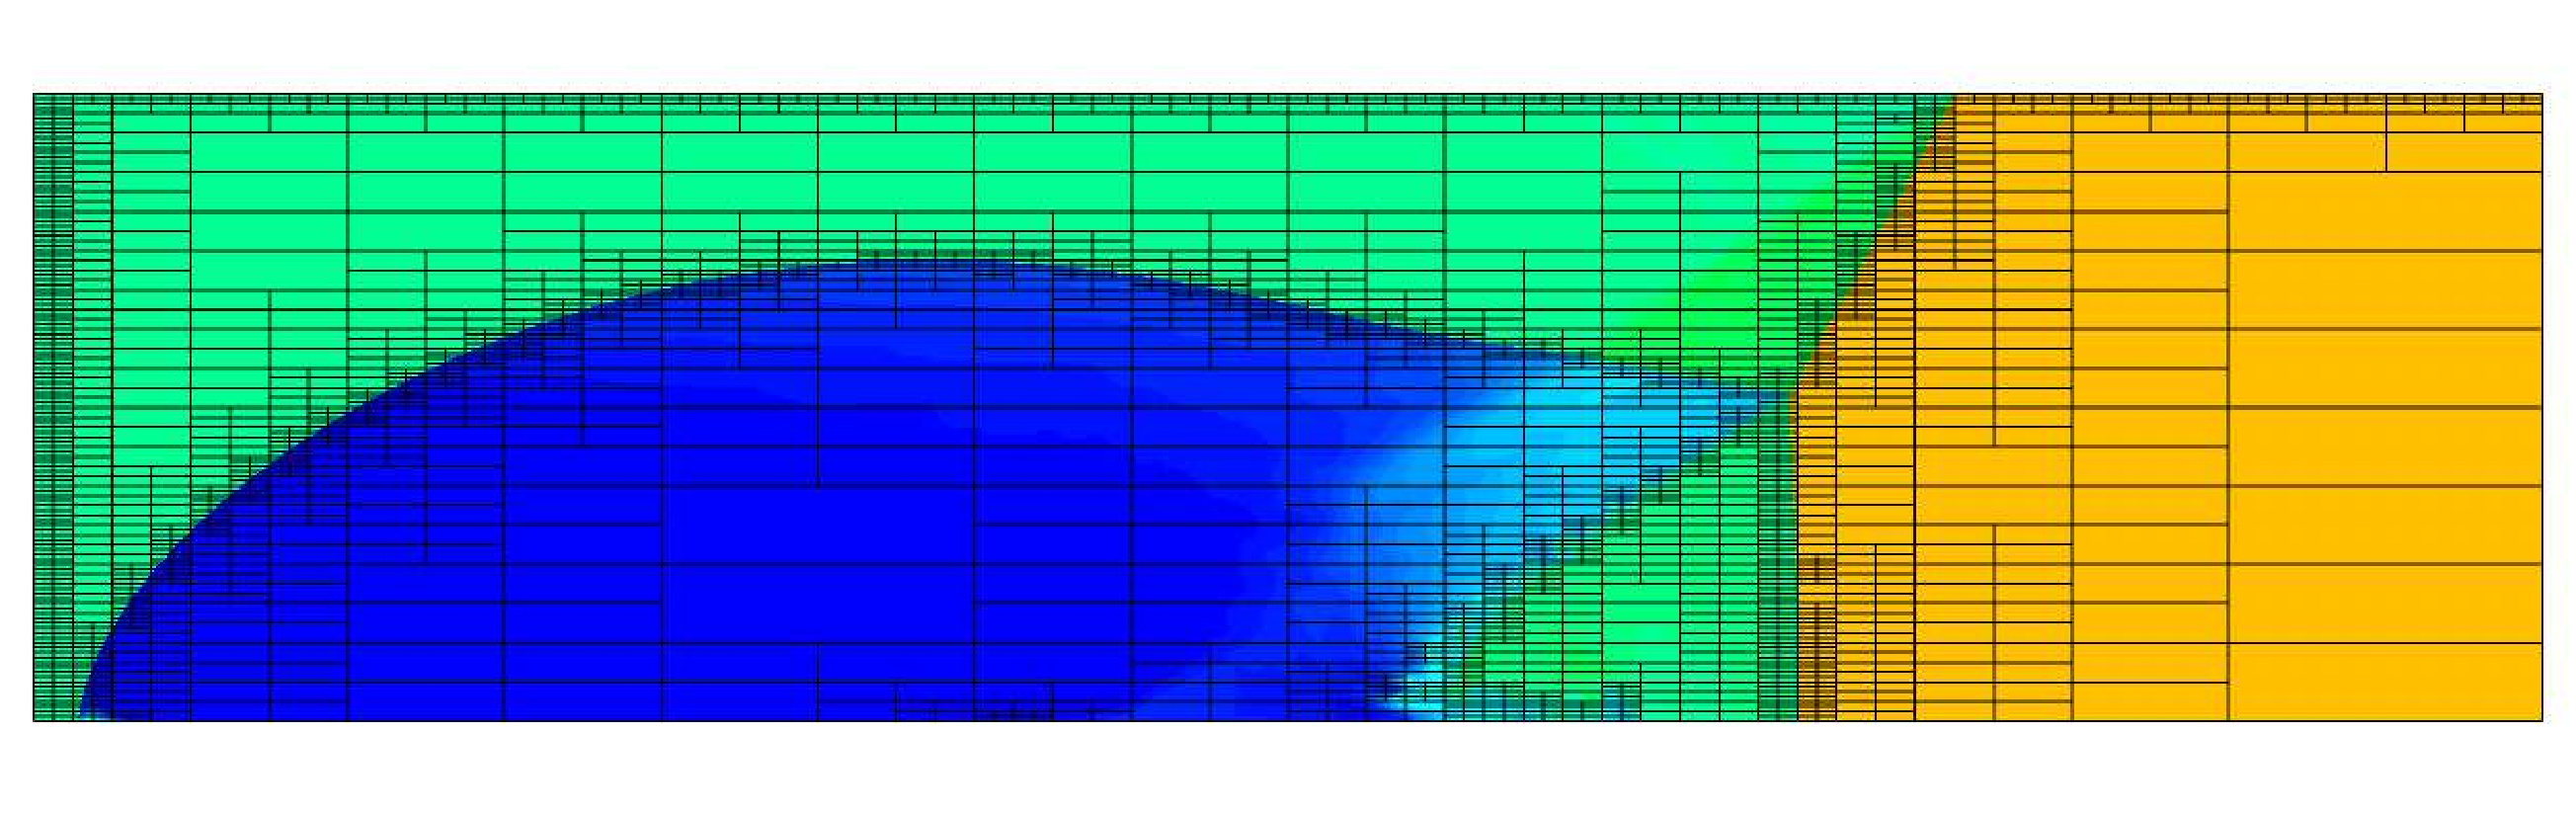
\includegraphics[width=8cm]{amr_demo}
\caption{7 levels of adaptive mesh refinement for a 2D integration.
}
\label{fig:3-7} % Give a unique label
\end{figure}

Simulations are by their nature only an approximation to reality.
To get closer to the real physics it is necessary to keep increasing the precision.
% Poorly resolved simulations can often provide misleading results.
Infinite precision would require an infinite number of computers, so we compromise by only requiring high precision in areas where the physics needs to be well followed. In the case of shock physics, the shocked regions require the highest precision and other regions where changes take place slowly and smoothly require lower precision.
A uniform high resolution or refinement is therefore a waste of limited and precious computing resources. 
A method of Adaptive Mesh Refinement (AMR) is used due to \citep{Berger84:_adapti,1989JCoPh..82...64B}, which allows the refined region to move with the shock. 
% Richardson truncation error estimation
There are several methods for determining whether it is necessary to refine or not.
One can refine 
\begin{itemize}
\item if the cell value is over a threshold.
\item By measuring the gradient of the solution, if it exceeds a predefined tolerance value the mesh is refined.
\item Richardson Truncation Error Estimation -- taking a short timestep at both the higher and lower levels and if the difference exceeds a certain tolerance, refining
\end{itemize}
% use a Richardson error estimation type method to determine the error.
In the wake of the shock the rest of the grid can use a lower level of resolution (derefine) and thus save on computing power. 
\begin{figure*}[t]
\centering
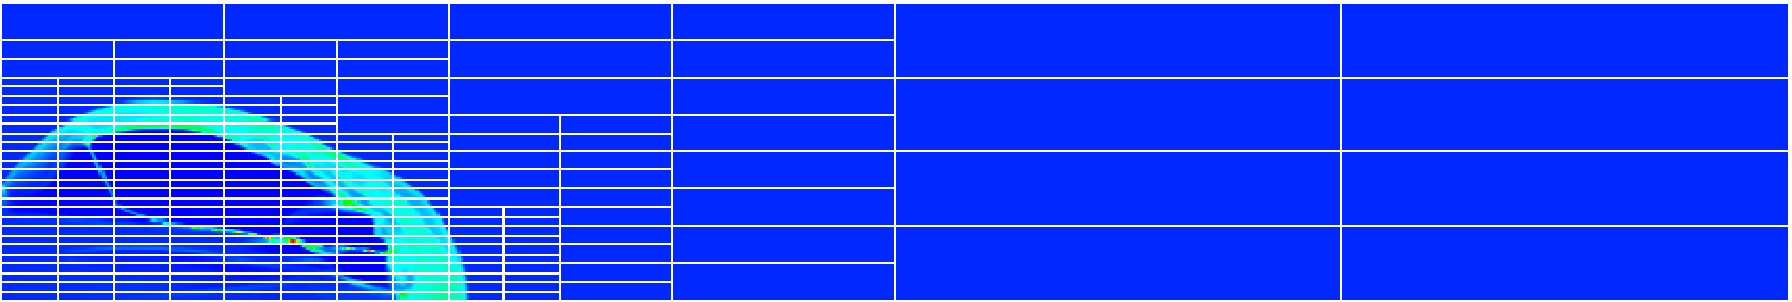
\includegraphics[width=15cm]{amr}
\caption{
Adaptive Mesh Refinement Example; this is an early stage of a 2D cylindrical symmetric jet simulation. Four levels of refinement are visible. The individual cells are not shown as they obscure the image - shown instead are the boundary boxes each of which bounds $10\mathrm{x}30$ cells.
}
\label{fig:2-3} % Give a unique label
\end{figure*}
ATLAS uses a library implementation of adaptive grids, PARAMESH, \citep{par:00} which is block-based -- the domain is partitioned into blocks of cells which are refined and derefined according to the amount of activity within the block. The mesh itself is structured -- cells do not change orientation or area. The co-ordinate system is Cartesian.
The adaptive grid methods used in PARAMESH represent several simplifications from the original method of \citet{Berger84:_adapti,1989JCoPh..82...64B} by disallowing change of orientation, overlapping, arbitrary shaping and merging. 
The justification for these changes is the simpler hierarchical structure which simply bisects grid blocks in each direction when refinement is required \citep{DeZeeuw93:_an_ada}.


%\subsection{Modifications and Additions Made to the Code}
%It was necessary to modify the code in several ways in order to model the jet more accurately. Added inflow boundary conditions, initial refinement at the inflow, added a module to account for the loss of energy due to cooling. Also had to write a new output method to produce ASCII output. 

%\subsection{Input/Output}
%Worker nodes report calculated results back to the master node.  This represents a break in the parallelism and a certain overhead in the runtime of the code -- however the alternative of parallel file output from each node is degrades performance even more.  Processing output data using a non-uniform mesh is not a straightforward operation.  The non-uniform data is not trivial to manipulate in 3D, and cannot be, for example, easily integrated without first paying attention to structure of the non-uniform mesh.  Standard visualisation tools such as MATLAB, IDL etc currently do not handle non-uniform data and unhappily a widely-used standard format for non-uniform data does not yet exist.  A dual approach was used -- visualisation and file storage were achieved using a modified version of the Hierarchical Data File system, formatted for use by the Chombo code to store non-uniform data.  This allowed data to be stored by block number rather than by grid reference and was compatible with the ChomboVis viewer.  Post-processing for integration required uniform data and this meant we had to either dump the data into a flat file and reassemble and refine it to a uniform level using a separate code.  Visualisation of the jet was done using ChomboVis. MPEG movies of the jet were created.  Some image processing was also done using ImageMagick and the GNU Image Manipulator.

\section{Leda, a parallel cluster}
In order to be able to run these simulations,
Stephane Dudzinski at the Dublin Institute for Advanced Studies and I built Leda, a parallel Beowulf-type cluster from computer parts.
The 16 dual-processor machines were hyperthreading enabled on each processor, which meant that the cluster had in total 64 processors.
The specifications are shown in Table \ref{tab:leda}.
Linux software was installed and message-passing software (the mpich package) was set up to allow communication between the nodes.
A gigabit star-topology ethernet connection was used to connect the nodes.
This cluster was used for much of the 1D and 2D simulation work in this thesis and also for the extinction mapping of the galactic plane.
Large-scale parallel simulations were done on the IBM SP5 in CINECA, the Irish
Centre for High End Computing (ICHEC)
Bull cluster ``Hamilton'' and the ICHEC Opteron cluster ``Walton'', the Trinity
College High Performance Computing
machine, and the ``Rowan'' EM64T cluster in University College Dublin.
Grid-based simulations were performed at 18 sites around Ireland using the Grid-Ireland system.

\begin{table}
\begin{tabular}{|p{3.5cm}|p{4.5cm}|p{4.5cm}|}
\hline
Nodes & \emph{Memory} & \emph{Speed}
\\
\hline
Worker & 512 MB& 2.66 GHz
\\
\hline
Master & 512 MB& 2.4 GHz
\\
\hline
\end{tabular}
\caption{Nodes on the Leda cluster}
\label{tab:leda}
\end{table}
